\chapter{Prototipo}\label{ch:prototipo}
Questo capitolo descriverà il progetto di prova finale realizzato durante il tirocinio. In particolare, si parlerà di ognuno dei tre livelli di sviluppo di un'applicazione web: il database, il back-end e il front-end e delle scelte progettuali fatte per realizzare il prototipo.

La parte di autenticazione all'applicazione web è stata gestita da \acrfull{gs} tramite un sistema di autenticazione di terze parti, in modo da poter gestire gli accessi e le autorizzazioni degli utenti in modo centralizzato, dai loro server esterni. Così facendo, il progetto non ha avuto necessità di sviluppare login e registrazione di utenti, ma si è concentrato sulle funzionalità di tracciamento e feedback delle attività formative erogate dall'azienda, in quanto la sicurezza di rete esulava dallo scopo del progetto di prova finale.\newline

% \begin{align}
TODO {\textbf{ mettere qui uno screen del prototipo finale}.}
% \end{align}

% DB %%%%%%%%%%%%%%%%%%%%%%%%%%%%%%%%%%%%%%%%%%%%%%%%%%%%%%%%%%%%%%%%%%%%%%%%%%%%%%%%%%%%%%%%%%%%%%%%%%%%%%%%
\newpage
\section{Database}\label{sec:database}
Innanzitutto è stato necessario progettare il database, nello specifico, è stato necessario creare le tabelle necessarie e riempirle con delle tuple\footnote{\glsdesc{tupla}} di prova per effettuare il giusto tracciamento del funzionamento e dei test del prototipo. 
Come da richiesta del tirocinio, le tabelle del database di gestione degli utenti non è stata realizzata, in quanto il progetto di tirocinio si è concentrato principalmente sulle funzionalità dell'amministratore e, quindi, il completo controllo -aggiungere, modificare, eliminare corsi formativi- delle attività formative erogate dall'azienda.

Il primo passo è stato quello di concepire le tabelle da integrare al \acrshort{db} già esistente -contenente le tabelle per la gestione di uffici e notiche di lavoro- e quindi fare le migrazioni\footnote{\glsdesc{migrazione}} necessarie. 

Grazie alle \acrshort{api} di \acrshort{asp.net}, è stato possibile creare e riempire le tabelle del database direttamente dal codice del backend, tramite le \acrfull{orm}, le quali si comportano come da ponte tra il codice e il \acrshort{db} relazionale. In pratica, è una tecnica per convertire i dati tra un \acrshort{db} relazionale e lo heap\footnote{\glsdesc{heap}} di un linguaggio di programmazione orientato agli oggetti (può anche essere vista come uno strato che collega la programmazione orientata agli oggetti coi \acrshort{db} relazionali). In questo specifico caso, non c'è stato bisogno di collegare le tabelle.
Nella sezione successiva (\ref{sec:backend}), vedremo l'implementazione nel dettaglio, senza alcun codice \acrshort{sql}.

Per la tabella dei corsi di formazione, sono stati creati i seguenti campi: 
\begin{itemize}
  \item \texttt{Id del corso} (integer), chiave primaria
  \item \texttt{CoursesName} (string), nome del corso
  \item \texttt{CoursesCapacity} (integer), capacità massima di utenti del corso
  \item \texttt{CoursesType} (string), tipologia del corso
  \item \texttt{CoursesDate} (string), data di inizio del corso
\end{itemize}

Una volta fatto ciò, la tabella che tiene traccia delle versioni del database, `VersionInfo' è stata aggiornata con le nuove migrazioni. Le sue colonne sono:
\begin{itemize}
  \item \texttt{Version} (integer), versione del database
  \item \texttt{AppliedOn} (datetime), data di applicazione della migrazione
  \item \texttt{Description} (text), descrizione della migrazione
\end{itemize}

Nella sezione successiva (\ref{sec:backend}) verranno analizzate nel dettaglio le porzioni di codice atte a creare la tabella \texttt{CoursesData} e a riempirla con delle tuple di prova.

Infine, per concludere questa sezione, per visualizzare e gestire il database, tramite \acrshort{gui}, è stato utilizzato DBeaver, un software gratuito e open source per la gestione di database relazionali, il quale ne supporta la maggior parte, come MySQL, PostgreSQL, Oracle, SQLite e SQL Server. La scelta è ricaduta su DBeaver per la sua semplicità d'uso e il fatto che sia sviluppato dalla comunità open source.
Il nome DBeaver deriva dalla combinazione di Database \acrshort{db} e Beaver, dall'inglese `castoro', una tra le tante legature di parole tipiche dell'informatica.

\begin{figure}[H]
\centering

\includegraphics[width=0.4\textwidth]{Images/dbeaver.png}
\caption{\label{fig:dbeaver}Il logo di DBeaver.}
\end{figure}


% backend %%%%%%%%%%%%%%%%%%%%%%%%%%%%%%%%%%%%%%%%%%%%%%%%%%%%%%%%%%%%%%%%%%%%%%%%%%%%%%%%%%%%%%%%%%%%%%%%%%%%
\newpage
\section{Backend}\label{sec:backend}
In questa sezione descriverò come ho usato \acrshort{asp.net} per lo sviluppo del back-end del progetto di prova finale.\newline

Lo sviluppo principale è stato fatto appoggiandosi all'applicazione web già esistente, sulla quale \acrfull{gs} ha sviluppato il progetto di tirocinio, che poi offre agli studenti. Quindi, basandomi sull'architettura già esistente, ho creato 5 nuove classi e modificato la classe \texttt{Program.cs}, già esistente, per gestire le funzionalità del prototipo. Queste classi sono:
\begin{itemize}
  \item \texttt{CoursesData.cs}
  \item \texttt{4\_CoursesMigration.cs}
  \item \texttt{CoursesController.cs}
  \item \texttt{CoursesDataGetListExecutor.cs}
  \item \texttt{CoursesDataExecuteExecutor.cs}
\end{itemize}

In particolare, la classe \texttt{CoursesData.cs} è stata creata per definire la tabella `CoursesData' e le sue colonne, tramite la libreria IdentityModel di \acrshort{asp.net}. La classe viene gestita come un'entità grazie all'attributo \texttt{[DbModel]} prima della sua definizione e le colonne vengono definite come proprietà\footnote{\glsdesc{proprietà}} della classe stessa -coi rispettivi getter\footnote{\glsdesc{getter}} e setter\footnote{\glsdesc{setter}}-, ognuna con un attributo loro attributo precedente che li definisce come proprietà \acrshort{json}, come si può vedere nel listato successivo (\ref{lst:coursesdata}); nella sezione successiva (\ref{sec:frontend}) verrà descritto nel dettaglio il loro funzionamento.\newline

\begin{figure}[H]
% \renewcommand{\lstlistingname}{Pippo}
\begin{lstlisting}[linewidth=20cm, caption={Il codice in C\# del file \texttt{CoursesData.cs}.}, captionpos=b, label={lst:coursesdata}]
  namespace It.gs.backend.Model
  {
  using System.Text.Json.Serialization;
  using It.gs.Repository;
  using It.gs.Repository.Model;

  public class AddCoursesToDbExecuteInfo : IExecuteInfo {
  public CoursesData[] Courses {get; set; }
  }
  public class DeleteCoursesDataExecuteInfo : IExecuteInfo {
  public CoursesData[] Courses {get; set; }
  }
  public class UpdateCoursesDataExecuteInfo : IExecuteInfo {
  public CoursesData[] Courses {get; set; }
  }
  [DbModel]
  public class CoursesData
  {
  [JsonPropertyName("coursesId")]
  public int CoursesId { get; set; }

  [JsonPropertyName("coursesName")]
  public string CoursesName { get; set; }

  [JsonPropertyName("coursesCapacity")]
  public int CoursesCapacity { get; set; }

  [JsonPropertyName("coursesType")]
  public string CoursesType { get; set; }

  [JsonPropertyName("coursesDate")]
  public string CoursesDate { get; set; }

  [JsonPropertyName("count")]
  public int? Count { get; set; }
  }
  }
\end{lstlisting}
\caption{\label{fig:coursesdata}Il codice in C\# del file \texttt{CoursesData.cs}.}
\end{figure}
\newpage

Analizzando nel dettaglio \texttt{4\_CoursesMigration.cs} invece, si può notare che è il file che contiene la creazione e la migrazione della tabella `CoursesData'. Di seguito, il listato (\ref{fig:coursemigration}) del codice in C\# del file:
\begin{figure}[H]
% \renewcommand{\lstlistingname}{Pippo}
\begin{lstlisting}[label={lst:coursemigration}, linewidth=20cm, basicstyle=\tiny]
namespace It.gs.backend.Migrations{
  using FluentMigrator; using It.gs.backend.Model;

  [Migration(4)] // Increment the db version, fourth migration
  public class CoursesMigration : Migration{
  public override void Down(){}
  public override void Up(){
  IfDatabase("sqlserver").Create.Schema("StarterDb");
  Create.Table($"{nameof(CoursesData)}")
  .WithColumn($"{nameof(CoursesData.CoursesId)}").AsInt32() .PrimaryKey().Identity()
  .WithColumn($"{nameof(CoursesData.CoursesName)}").AsString() .NotNullable().WithDefaultValue(false)
  .WithColumn($"{nameof(CoursesData.CoursesCapacity)}") .AsInt16().NotNullable().WithDefaultValue(10)
  .WithColumn($"{nameof(CoursesData.CoursesType)}").AsString() .NotNullable()
  .WithColumn($"{nameof(CoursesData.CoursesDate)}").AsString() .NotNullable();
  var coursesRows = new List<dynamic>{
  new { CoursesId = 1, CoursesName = "Angular Modulo 1", CoursesCapacity = 10, CoursesType = "Udemy",CoursesDate = "30-01-2024" },
  new { CoursesId = 2, CoursesName = "Angular Modulo 2", CoursesCapacity = 10, CoursesType = "Udemy",  CoursesDate = "30-02-2024" },
  new { CoursesId = 3, CoursesName = "Angular Modulo 3", CoursesCapacity = 10, CoursesType = "Udemy",  CoursesDate = "30-03-2024" },
  new { CoursesId = 4, CoursesName = "Angular Modulo 4", CoursesCapacity = 10, CoursesType = "Udemy",  CoursesDate = "30-04-2024" },
  new { CoursesId = 5, CoursesName = "Angular Modulo 5", CoursesCapacity = 10, CoursesType = "Udemy",  CoursesDate = "30-05-2024" },
  };
  foreach(var course in coursesRows)
  Insert.IntoTable($"{nameof(CoursesData)}").Row(course);
  // Delete.Table($"{nameof(CoursesData)}");
  }
  }
}
\end{lstlisting}
\caption{\label{fig:coursemigration}Il codice in C\# del file \texttt{4\_CoursesMigration.cs}.}
\end{figure}
Grazie alla libreria FluentMigrator di \gls{.net}, ho potuto creare la tabella `CoursesData' e riempirla con le tuple di prova precedentemente citate. È ovviamente importante ricordarsi di estendere la classe \texttt{Migration} e di implementare i metodi \texttt{Down ()} e \texttt{Up ()}, altrimenti il codice non funzionerebbe. Inoltre, in questo caso, è anche necessario tener traccia della versione del \acrshort{db}, incrementando di volta in volta il numero della migrazione, come si può notare dall'attributo \texttt{[Migration ()]} a cui viene passato l'intero numero 4.
I metodi \texttt{Up ()} e \texttt{Down ()} si occupano rispettivamente di `spostare' il \acrshort{db} in avanti e indietro nelle migrazioni, a un qualsiasi punto nel tempo. L'unico accorgimento è che la migrazione all'indietro è distruttiva, in quanto le tabelle o le righe vengono eliminate nel processo. È quindi necessario e consigliabile fare preventivamente un backup\footnote{\glsdesc{backup}}, se si vuole essere sicuri di mantenere i dati.

Analizzando nel dettaglio la porzione di codice del metodo \texttt{Up ()}, si può notare che, riguarda la creazione della tabella \texttt{CoursesData}: innanzitutto crea uno schema -\texttt{StarterD}- e controlla che sia effettivamente un \acrshort{db} \acrshort{sql}Server. Una volta sicuro, crea la tabella \texttt{CoursesData} e le sue colonne, specificandone il tipo e se sono o meno nullabili, in particolare:
\begin{itemize}
  \item Il metodo \texttt{AsInt16} sta per `integer a 16 bit', ovvero un intero a 2 byte;
  \item Il metodo \texttt{AsInt32} sta per `integer a 32 bit', ovvero un intero a 4 byte;
  \item Il metodo \texttt{AsString} comunica al \acrshort{db} che il campo su cui è chiamato sarà di tipo stringa;
  \item Il metodo \texttt{NotNullable} stabilisce che il campo non può essere nullo;
  \item Il metodo \texttt{WithDefaultValue} stabilisce il valore di default del campo, in questo caso \texttt{false}, ma ovviamente accetta anche \texttt{true} come parametro;
  \item Il metodo \texttt{PrimaryKey} stabilisce che il campo è una chiave primaria;
  \item Il metodo \texttt{Identity} stabilisce che il campo su cui è chiamato è un campo identità, ciò significa che il valore per questo campo sarà automaticamente generato dal \acrshort{db} e sarà incrementato di volta in volta.
\end{itemize}

Successivamente, viene creata una lista dinamica in cui vengono inserite le righe di prova, coi valori dei campi corrispondenti. Infine, viene fatto un ciclo \texttt{foreach} in cui, per ogni riga della lista, viene inserita una riga nella tabella \texttt{CoursesData}.

Durante lo sviluppo del prototipo, si è presentata la necessità di cancellare la tabella \texttt{CoursesData} per debuggare il codice, ecco il motivo della riga 24 commentata.

Passando invece al file \texttt{CoursesController.cs}, si può notare che è stato creato per gestire le richieste \acrshort{http} relative ai corsi di formazione. Di seguito, il listato (\ref{fig:coursescontroller}) del codice in C\# del file:
\begin{figure}[H]
  % \renewcommand{\lstlistingname}{Pippo}
\begin{lstlisting}[linewidth=100cm]
[Route("api/v{version:apiVersion}/[controller]")]
[ApiController]
[ApiVersion("1.0")]
[Authorize(Policy = Policies.Base)]
public class CoursesController : ControllerBase{
  private readonly IRepositoryModule<CoursesData> coursesDataRepo;
  public CoursesController(IRepositoryModule<CoursesData>    CoursesDataRepo) { this.coursesDataRepo = CoursesDataRepo; }

  [HttpPost("searchCoursesData")]
  [ProducesResponseType(typeof(CoursesData[]), 200)] ... (400) ... (500)
  public async Task<IActionResult> SearchCoursesData([FromBody] DynamicQueryPart query) =>
  await GetList<CoursesData>( e => StatusCode(500, e), v => Ok(v), Maybe<CoreDynamicQueryPart>.From(query))();
  
  [HttpPost("addCoursesData")]
  [ProducesResponseType(200)] ... (400) ... (500)
  public async Task<IActionResult> AddCoursesToDb([FromBody]   CoursesData[] Courses) {
  var CoursesInfo = new AddCoursesToDbExecuteInfo {Courses = Courses};
  var result = await this.coursesDataRepo.Execute(CoursesInfo);
  if(result.IsSuccess) return Ok();
  else throw result.Error.SourceException;
  }

  [HttpDelete("deleteCoursesData/{CoursesId}")]
  [ProducesResponseType(200)] ... (400) ... (500)
  public async Task<IActionResult> DeleteCoursesData(int CoursesId) {
  var CoursesInfo = new DeleteCoursesDataExecuteInfo{Courses=new[]{new CoursesData { CoursesId = CoursesId } } };
  var result = await this.coursesDataRepo.Execute(CoursesInfo);
  if (result.IsSuccess) return Ok();
  else throw result.Error.SourceException;
  }
  
  [HttpPut("updateCoursesData")] ... [ProducesResponseType(... ... ...)]
  public async Task<IActionResult>UpdateCoursesData([FromBody]  CoursesData[] Courses) {
  var CoursesInfo = new UpdateCoursesDataExecuteInfo{Courses = Courses};
  var result = await this.coursesDataRepo.Execute(CoursesInfo);
  if (result.IsSuccess) return Ok();
  else throw result.Error.SourceException;
  }  
}
\end{lstlisting}
\caption{\label{fig:coursescontroller}Il codice in C\# del file \texttt{CoursesController.cs}.}
\end{figure}
\textbf{Nota che } alcuni attrubuti sono stati sostituiti con dei puntini, per motivi di spazio e per ridondanza (l'unico cambiamento è il parametro, -200, 400 o 500- il resto è identico) e che il \texttt{namespace} e gli \texttt{using} sono stati omessi per gli stessi motivi. 

La classe mostrata precendentemente (\ref{fig:coursescontroller}), necessita di estendere la classe \texttt{ControllerBase} per poter gestire le richieste \acrshort{http} citate sopra. Altri dettagli degni di nota sono:
\begin{itemize}
  \item L'attributo \texttt{[Route ()]} specifica il percorso della richiesta \acrshort{http} e il numero di versione dell'\acrshort{api};
  \item L'attributo \texttt{[Authorize ()]} specifica una politica di autorizzazione, in questo caso \texttt{Policies.Base};
  \item Tutti i metodi sono asincroni, in quanto si aspettano una risposta dal \acrshort{db} e, quindi, non possono bloccare il processo principale;
  \item Il metodo \texttt{SearchCoursesData ()} è preceduto dall'attributo \texttt{[HttpPost ()]}, il quale specifica che la richiesta \acrshort{http} sarà di tipo \texttt{POST}, dal nome `searchCoursesData' e dall'attributo \texttt{[ProducesResponseType ()]}, il quale stabilisce che la risposta del metodo sarà un array di tipo \texttt{CoursesData}, con codice di stato 200, 400 o 500;
  \item Analogamente per gli altri metodi, \texttt{AddCoursesToDb ()}, \texttt{DeleteCoursesData ()} e \texttt{UpdateCoursesData ()}, con la differenza che `updateCoursesData' userà il metodo \acrshort{http} \texttt{PUT} e `deleteCoursesData' userà il metodo \acrshort{http} \texttt{DELETE}.
\end{itemize}
A questo punto, \texttt{CoursesDataExecuteExecutor.cs} si occupa di eseguire l'operazione richiesta (richiesta o risposta \acrshort{http}), le quali sono state definite dal `controller' descritto sopra.
Qui di seguito, il listato (\ref{fig:coursesdataexecuteexecutor}) del codice in C\# del file `Executor':
\begin{figure}[H]
  % \renewcommand{\lstlistingname}{Pippo}
\begin{lstlisting}[label={lst:coursesdataexecuteexecutor}, linewidth=20cm, basicstyle=\tiny]
  public class CoursesDataExecuteexecutor_: IExecuteWithTransactionExecutor<CoursesData>
  {
  // ...
  }
\end{lstlisting}
\caption{\label{fig:coursesdataexecuteexecutor}Il codice in C\# della classe di \texttt{CoursesDataExecuteExecutor.cs}, successivamente diviso in blocchi di codice per motivi di spazio.}
\end{figure}

\begin{figure}[H]
% \renewcommand{\lstlistingname}{Pippo}
\begin{lstlisting}[linewidth=20cm, basicstyle=\tiny]
public async Task<IExecuteResult> Execute(DatabaseSettings settings, IDbConnection connection, IDbTransaction transaction, IExecuteInfo info)
{
  switch(info) {
  case AddCoursesToDbExecuteInfo i: 
   return await AddCoursesExecute(settings, connection, transaction, i);
  case DeleteCoursesDataExecuteInfo i:
   return await DeleteCoursesDataExecute(settings, connection, transaction, i);
  case UpdateCoursesDataExecuteInfo i:
   return await UpdateCoursesDataExecute(settings, connection, transaction, i);
  default: throw new NotSupportedException($"Execute with transaction for type {info.GetType().FullName} not supported");
  }
}
private async Task<IExecuteResult> AddCoursesExecute(DatabaseSettings settings, IDbConnection connection, IDbTransaction transaction, AddCoursesToDbExecuteInfo info) {
  foreach(var Course in info.Courses)
  _ = await Add(settings, connection, transaction, Course);
  return await IExecuteResult.From(true);
}
private async Task<CoursesData> Add(DatabaseSettings settings, IDbConnection connection, IDbTransaction transaction, CoursesData item)
{
  Console.WriteLine("item: ",item);
  var sql = $"INSERT INTO CoursesData (CoursesName, CoursesCapacity, CoursesType, CoursesDate) VALUES (@{nameof(CoursesData.CoursesName)}, @{nameof(CoursesData.CoursesCapacity)}, @{nameof(CoursesData.CoursesType)}, @{nameof(CoursesData.CoursesDate)})";

  var r = await connection.ExecuteAsync(sql, item, transaction);
  return item;
}
\end{lstlisting}
\caption{\label{fig:executor_add}Il codice di \texttt{CoursesDataExecuteExecutor.cs}, relativo alla scelta del metodo e all'aggiunta delle tuple.}
\end{figure}

\begin{figure}[H]
\begin{lstlisting}[label={lst:executor_delete}, linewidth=20cm, basicstyle=\tiny]
private async Task<IExecuteResult> DeleteCoursesDataExecute(DatabaseSettings settings, IDbConnection connection, IDbTransaction transaction, DeleteCoursesDataExecuteInfo info) {
  foreach(var Course in info.Courses)
  _ = Remove(settings, connection, transaction, Course);

  return await IExecuteResult.From(true);
}
private async Task<CoursesData> Remove(DatabaseSettings settings, IDbConnection connection, IDbTransaction transaction, CoursesData item)
{  
  var sql = $"DELETE FROM CoursesData WHERE CoursesId = @CoursesId";

  var affectedRows = await connection.ExecuteAsync(sql, new { CoursesId = item.CoursesId }, transaction);
  var r = await connection.ExecuteAsync(sql, item, transaction);
  return item;
}
\end{lstlisting}
\caption{\label{fig:executor_delete}Il codice di \texttt{CoursesDataExecuteExecutor.cs}, relativo alla cancellazione delle tuple.}
\end{figure}

\begin{figure}[H]
\begin{lstlisting}[linewidth=20cm, basicstyle=\tiny]
private async Task<IExecuteResult> UpdateCoursesDataExecute(DatabaseSettings settings, IDbConnection connection, IDbTransaction transaction, UpdateCoursesDataExecuteInfo info) {
  foreach(var Course in info.Courses)
  _ = await Update(settings, connection, transaction, Course);

  return await IExecuteResult.From(true);
}
private async Task<CoursesData> Update(DatabaseSettings settings, IDbConnection connection, IDbTransaction transaction, CoursesData item)
{
  var sql = 
  $"UPDATE {nameof(CoursesData)} " +
  $"SET " +
  $"{nameof(CoursesData.CoursesName)} = @{nameof(CoursesData.CoursesName)}, " +
  $"{nameof(CoursesData.CoursesCapacity)} = @{nameof(CoursesData.CoursesCapacity)}, " +
  $"{nameof(CoursesData.CoursesType)} = @{nameof(CoursesData.CoursesType)}, " +
  $"{nameof(CoursesData.CoursesId)} = @{nameof(CoursesData.CoursesId)}, " +
  $"{nameof(CoursesData.CoursesDate)} = @{nameof(CoursesData.CoursesDate)} " +
  $"WHERE {nameof(CoursesData.CoursesId)} = @{nameof(CoursesData.CoursesId)}";

  var r = await connection.ExecuteAsync(sql, item, transaction);
  return item;
}
\end{lstlisting}
\caption{\label{fig:executor_update}Il codice di \texttt{CoursesDataExecuteExecutor.cs}, relativo all'aggiornamento delle tuple.}
\end{figure}

La classe \texttt{CoursesDataExecuteExecutor.cs}, come possiamo vedere dai listati soprastanti, smista la richiesta grazie ai parametri passati. In particolare tramite il parametro \texttt{info}, è in grado di eseguire il giusto metodo per ogni tipologia richiesta.
Ognuno dei metodi ausiliari \texttt{AddCoursesExecute ()}, \texttt{DeleteCoursesDataExecute ()} e \texttt{UpdateCoursesDataExecute ()} si occupa di chiamare i rispettivi metodi \texttt{Add ()}, \texttt{Remove ()} e \texttt{Update ()}, usando i parametri corretti; questi ultimi invece, imposteranno le query corrette per ogni tipo di operazione richiesta, come si può notare dai listati (\ref{fig:executor_add}), (\ref{fig:executor_delete}) e (\ref{fig:executor_update}), per poi chiamare il metodo \texttt{ExecuteAsync ()}, il quale esegue effettivamente la query, infatti, \texttt{ExecuteAsync ()} è un metodo asincrono, in quanto si aspetta una risposta dal \acrshort{db} e, quindi, non può bloccare il processo principale. 
Inoltre, è un metodo che restituisce un oggetto di tipo \texttt{Task}, il quale rappresenta un'operazione, semppre asincrona, che può restituire un valore, in questo caso un oggetto di tipo \texttt{IExecuteResult}, il quale rappresenta il risultato dell'operazione.\newline

È degno di nota anche il file \texttt{CoursesDataGetListExecutor.cs}, il quale si occupa di raccogliere la lista dei corsi di formazione, tramite il metodo \texttt{GetList ()}, chiamato dalla classe \texttt{CoursesController} descritta in precedenza. Di seguito, il listato (\ref{fig:get list}) del codice in C\# del file:
\begin{figure}[H]
\begin{lstlisting}[linewidth=20cm, basicstyle=\tiny]
  public class CoursesDataGetListexecutor_: IGetListExecutor<CoursesData>, IAddExecutor<CoursesData>
  {
  public async Task<CoursesData> Add(DatabaseSettings settings, IDbConnection connection, IDbTransaction transaction, CoursesData item)
  {
   var sql = $"INSERT INTO CoursesData (CoursesName, CoursesCapacity, CoursesType, CoursesDate) VALUES (@{nameof(CoursesData.CoursesName)}, @{nameof(CoursesData.CoursesCapacity)}, @{nameof(CoursesData.CoursesType)}, @{nameof(CoursesData.CoursesDate)})";

   var r = await connection.ExecuteAsync(sql, item, transaction);
   if(r > 0) return item;
   else throw new InvalidOperationException("ERROR!!!");
  }

  public async Task<IEnumerable<CoursesData>> GetList(DatabaseSettings settings, IDbConnection connection,  Maybe<CoreDynamicQueryPart> query)
  {
   var (countSql, sql, parameters) = query.EnsureOrderBy(nameof(CoursesData.CoursesId)) .ComposeWithCount<DapperQueryParametersBuilder, DynamicParameters>($"SELECT * $FROM{nameof(CoursesData)}"  , nameof(CoursesData.CoursesId), settings);
   var result = await connection.QueryAsync<CoursesData>(sql: sql, param: parameters);
   var count = await connection.QuerySingleAsync<int>(sql:  countSql, param: parameters);
   return result.Select(x => { x.Count = count; return x; });
  }
  }
\end{lstlisting}
\caption{\label{fig:get list}Il codice di \texttt{CoursesDataGetListExecutor.cs}, classe contenente il metodo \texttt{GetList ()}.}
\end{figure}
Si nota l'implementazione di un altro metodo \texttt{Add ()}: le differenze con il metodo \texttt{Add ()} della classe \texttt{CoursesDataExecuteExecutor.cs} sono minime, in quanto entrambi eseguono una query di inserimento, ma per la classe (\ref{fig:get list}) è un metodo pubblico, il quale effettua anche un controllo sull'esito dell'operazione, restituendo un'eccezione in caso negativo.
È importante notare che la classe \texttt{CoursesDataGetListExecutor} usa la libreria Dapper, una micro \acrshort{orm} per interagire con il \acrshort{db}. Infatti, Dapper mappa i risultati delle query \acrshort{sql} in oggetti C\#, il che rende più facile lavorare con i dati relazionali risultanti.\newline

Infine, è stato necessario configurare il file principale \texttt{Program.cs}, aggiungendogli le righe di codice relative alle nuove classi e ai loro metodi. La prima build\footnote{\glsdesc{build}} del backend era pronta.\newline

A questo punto, era necessario testare che l'implementazione del backend funzionasse correttamente. Ho utilizzato una \acrshort{api} apposita, Swagger.

\subsection{Swagger}\label{subsec:swagger}
\begin{figure}[H]
\centering

\includegraphics[width=0.4\textwidth]{Images/Swagger-logo.png}
\caption{\label{fig:swaggerlogo}Il logo di Swagger.}
\end{figure}

Swagger è un insieme di strumenti per sviluppatori di \acrshort{api}, originariamente specificata e sviluppata da SmartBear Software, nel 2011. 
In questo caso, il suo utilizzo è stato principalmente quello di testare il corretto funzionamento del backend. Il suo vantaggio principale sta nella possibilità di utilizzarlo direttamente dal browser, senza dover installare alcun software aggiuntivo, è sufficiente digitare un indirizzo \acrshort{url} apposito -per esempio \texttt{https://localhost:5001/swagger/index.html}- e si aprirà una pagina web con un'interfaccia grafica dedicata, in cui ci sarà una lista di tutte le \acrshort{api} disponibili, sviluppate con \acrshort{asp.net}.
\begin{figure}[H]
\centering
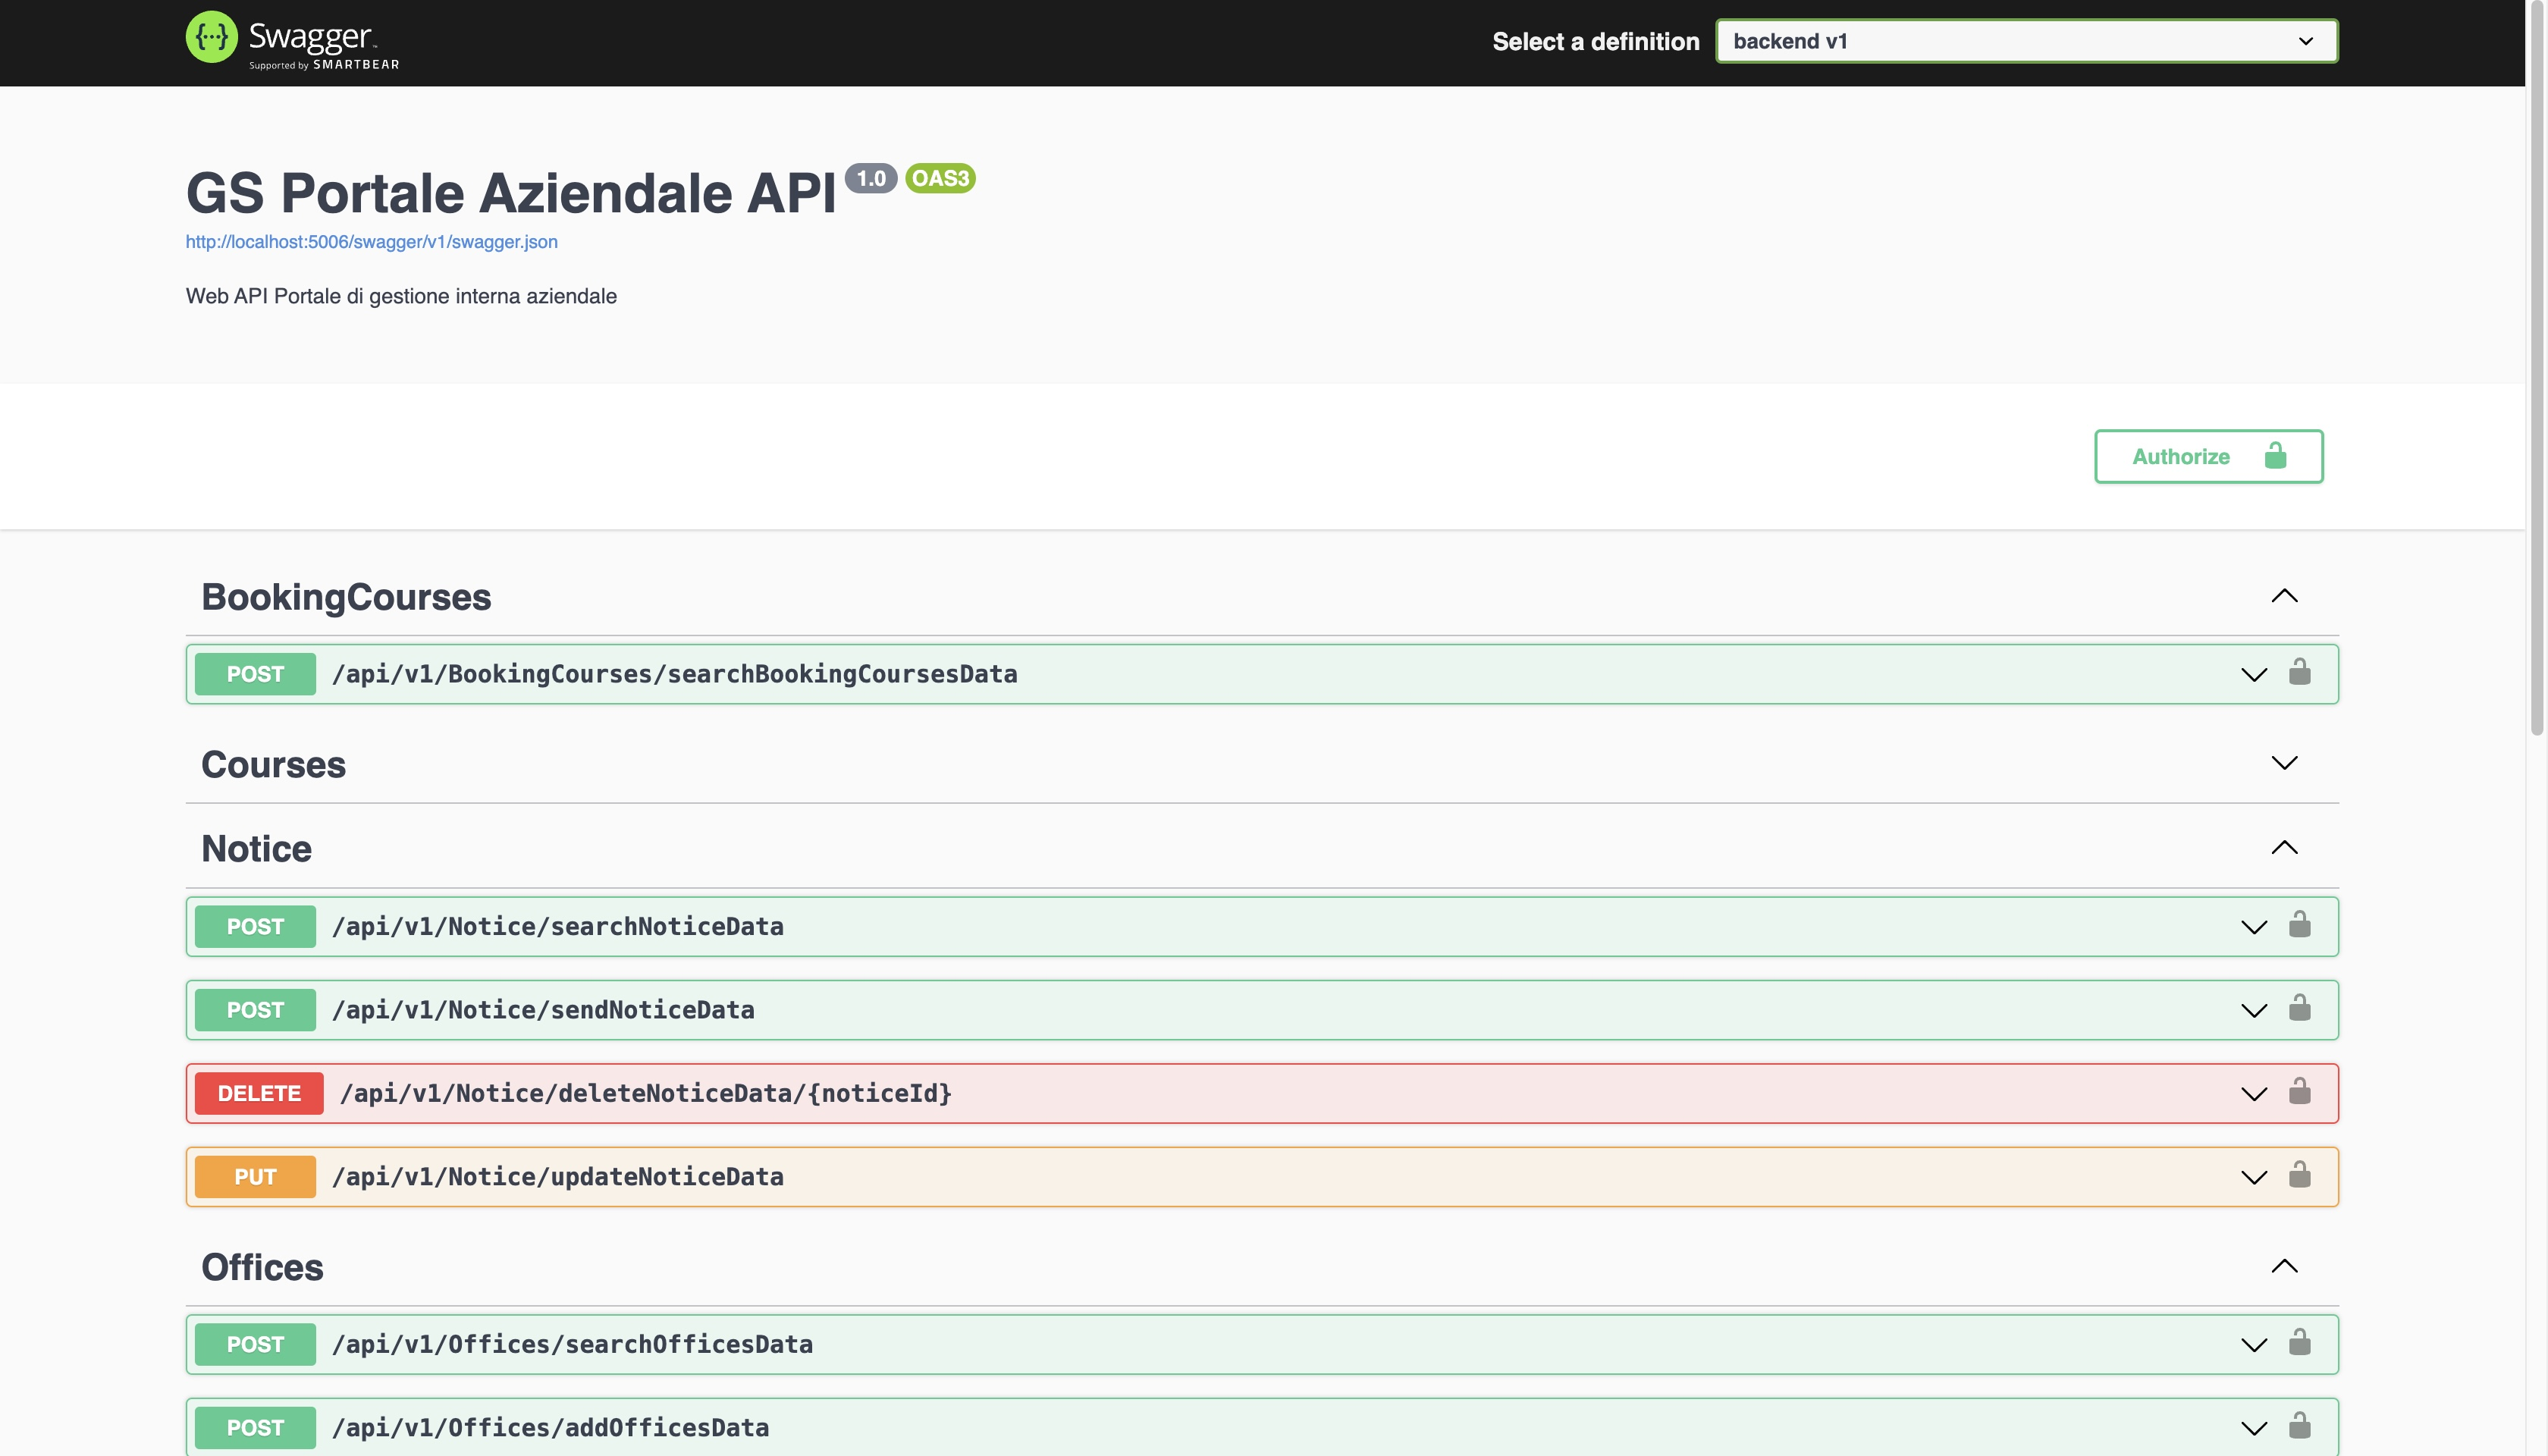
\includegraphics[width=1\textwidth]{Images/swagger.jpg}
\caption{\label{fig:swagger}L'interfaccia grafica di Swagger, relativa al progetto di tirocinio.}
\end{figure}
Una volta autenticatosi con le giuste credenziali -nel mio caso, quelle fornite da \acrlong{gs}-, si ha l'autorizzazione necessaria per poter eseguire le \acrshort{api} sviluppate. Di seguito alcuni esempi di esecuzione e del loro risultato:
\begin{figure}[H]
\centering
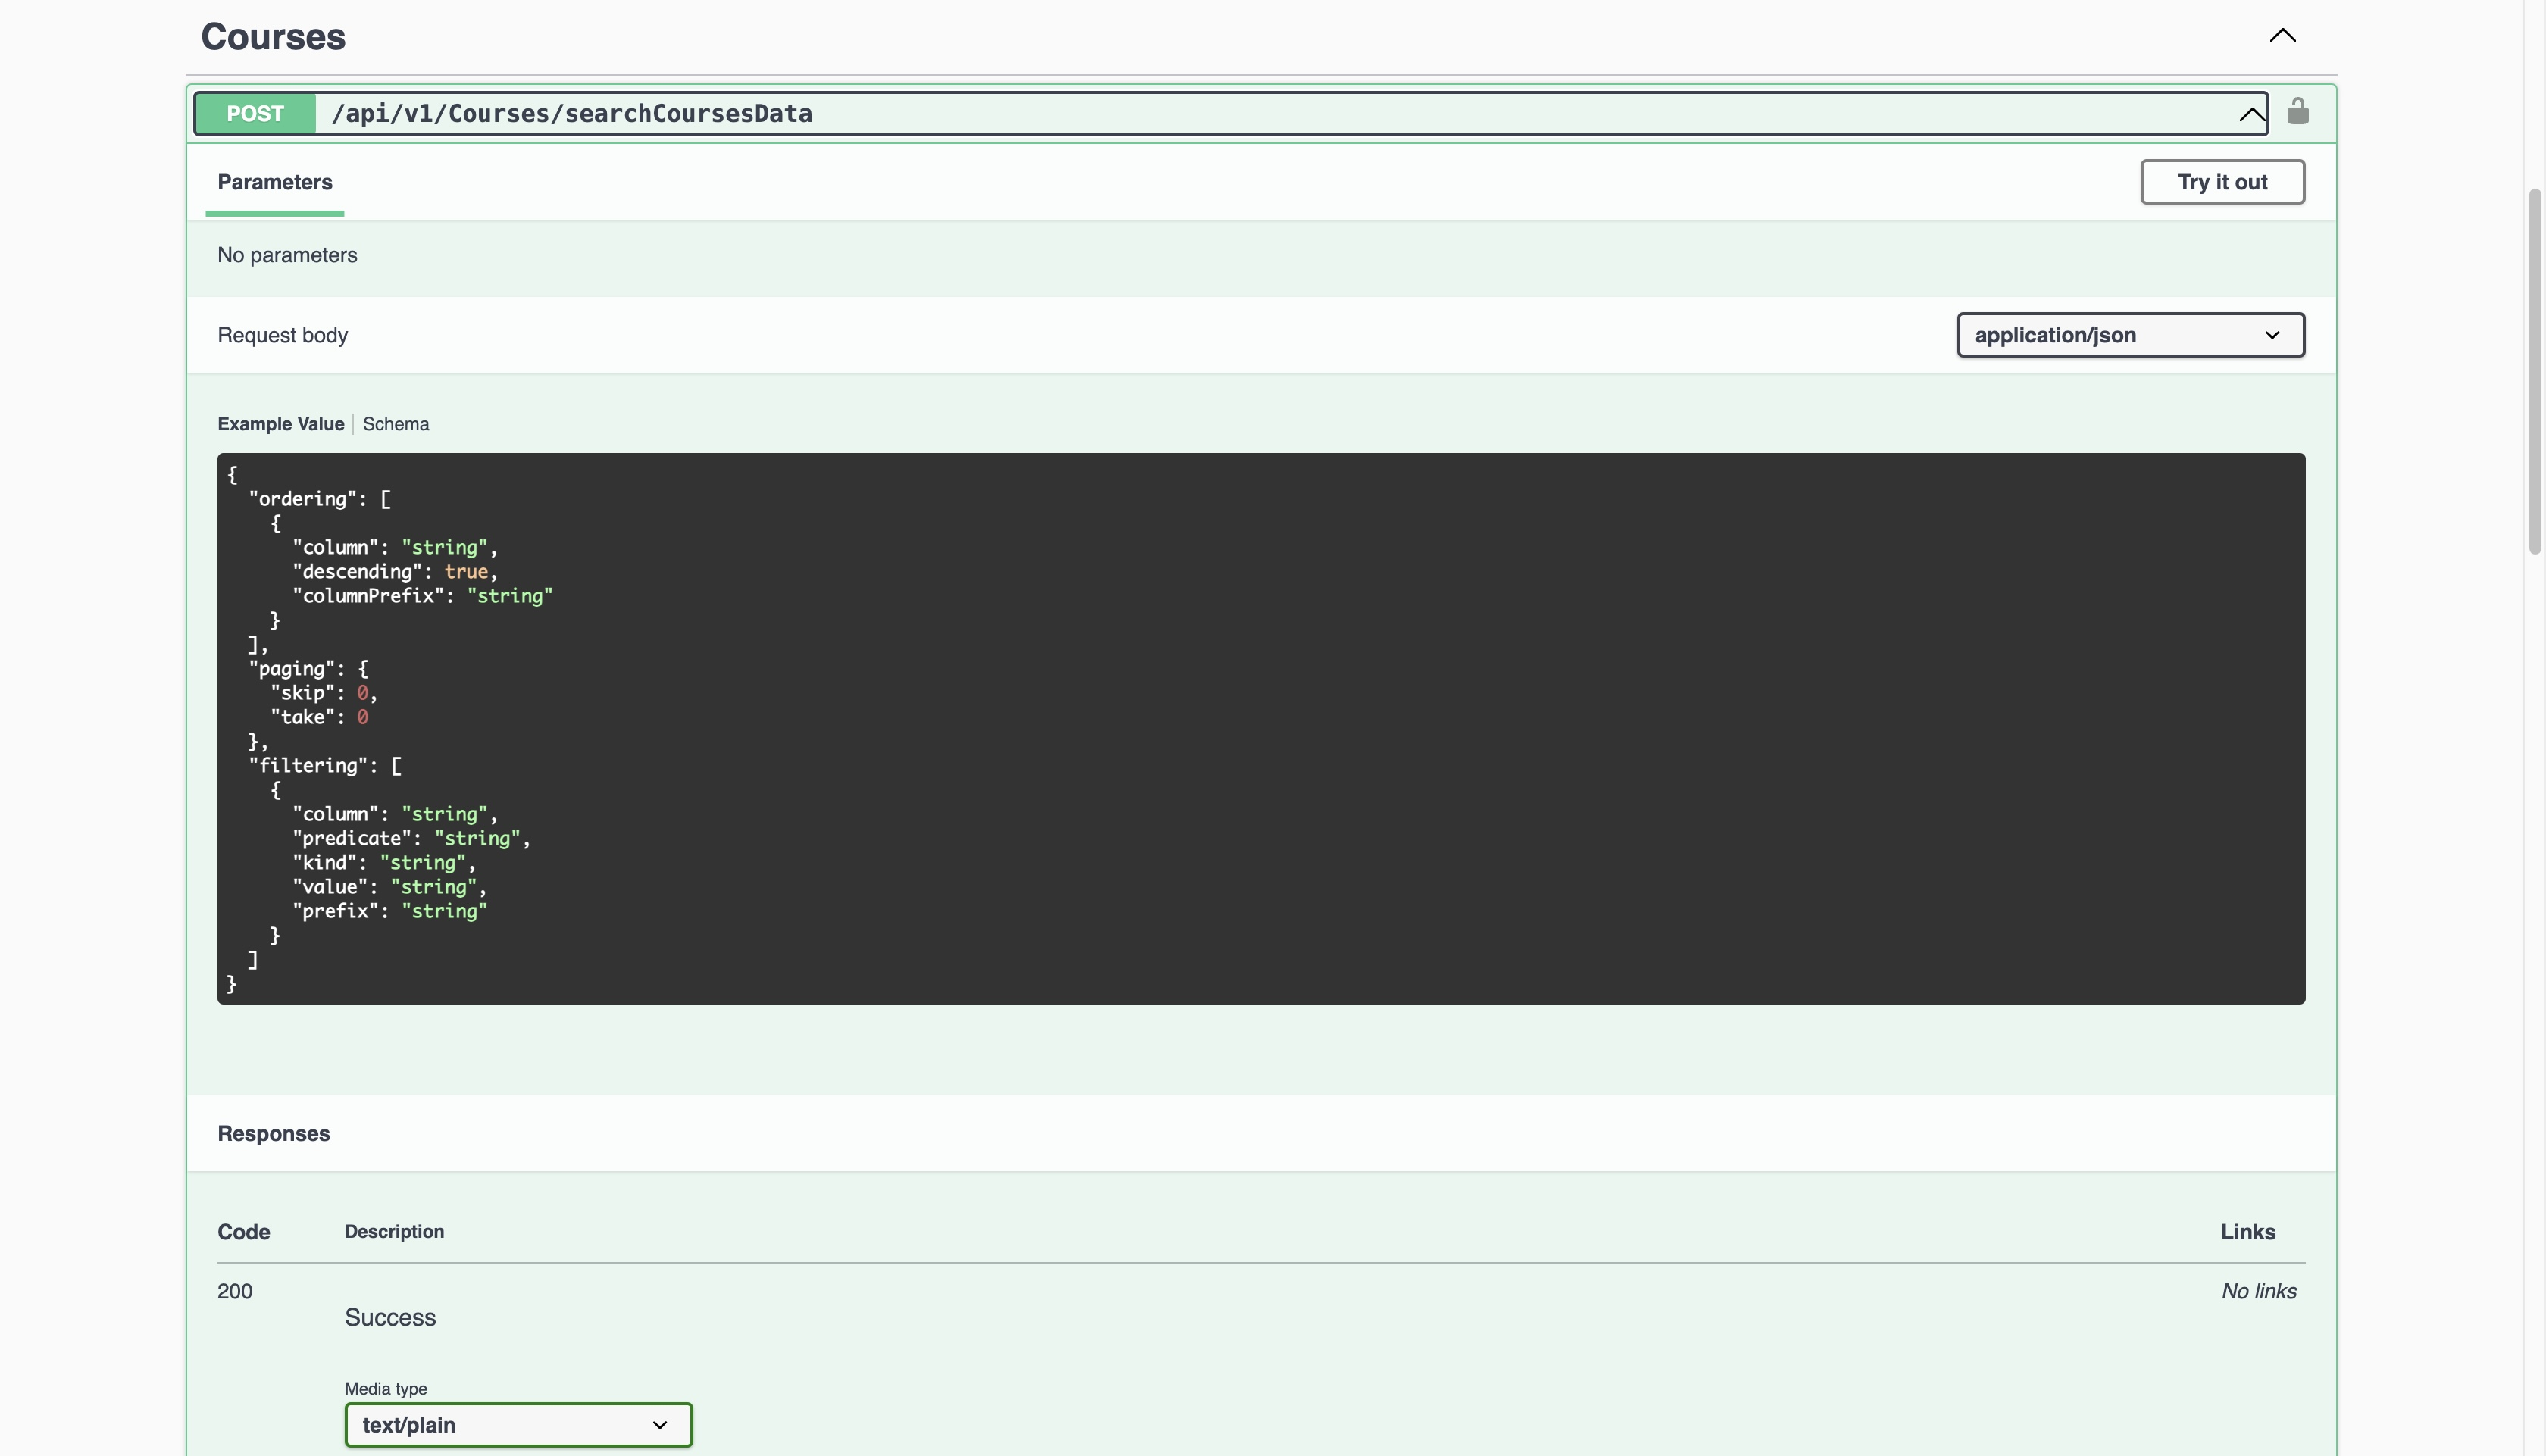
\includegraphics[width=1\textwidth]{Images/swagger courses.jpg}
\caption{\label{fig:swagger courses}Esempio di esecuzione di una \acrshort{api} per \texttt{searchCoursesData}, il corpo della richiesta è in formato \acrshort{json}.}
\end{figure}

\begin{figure}[H]
\centering
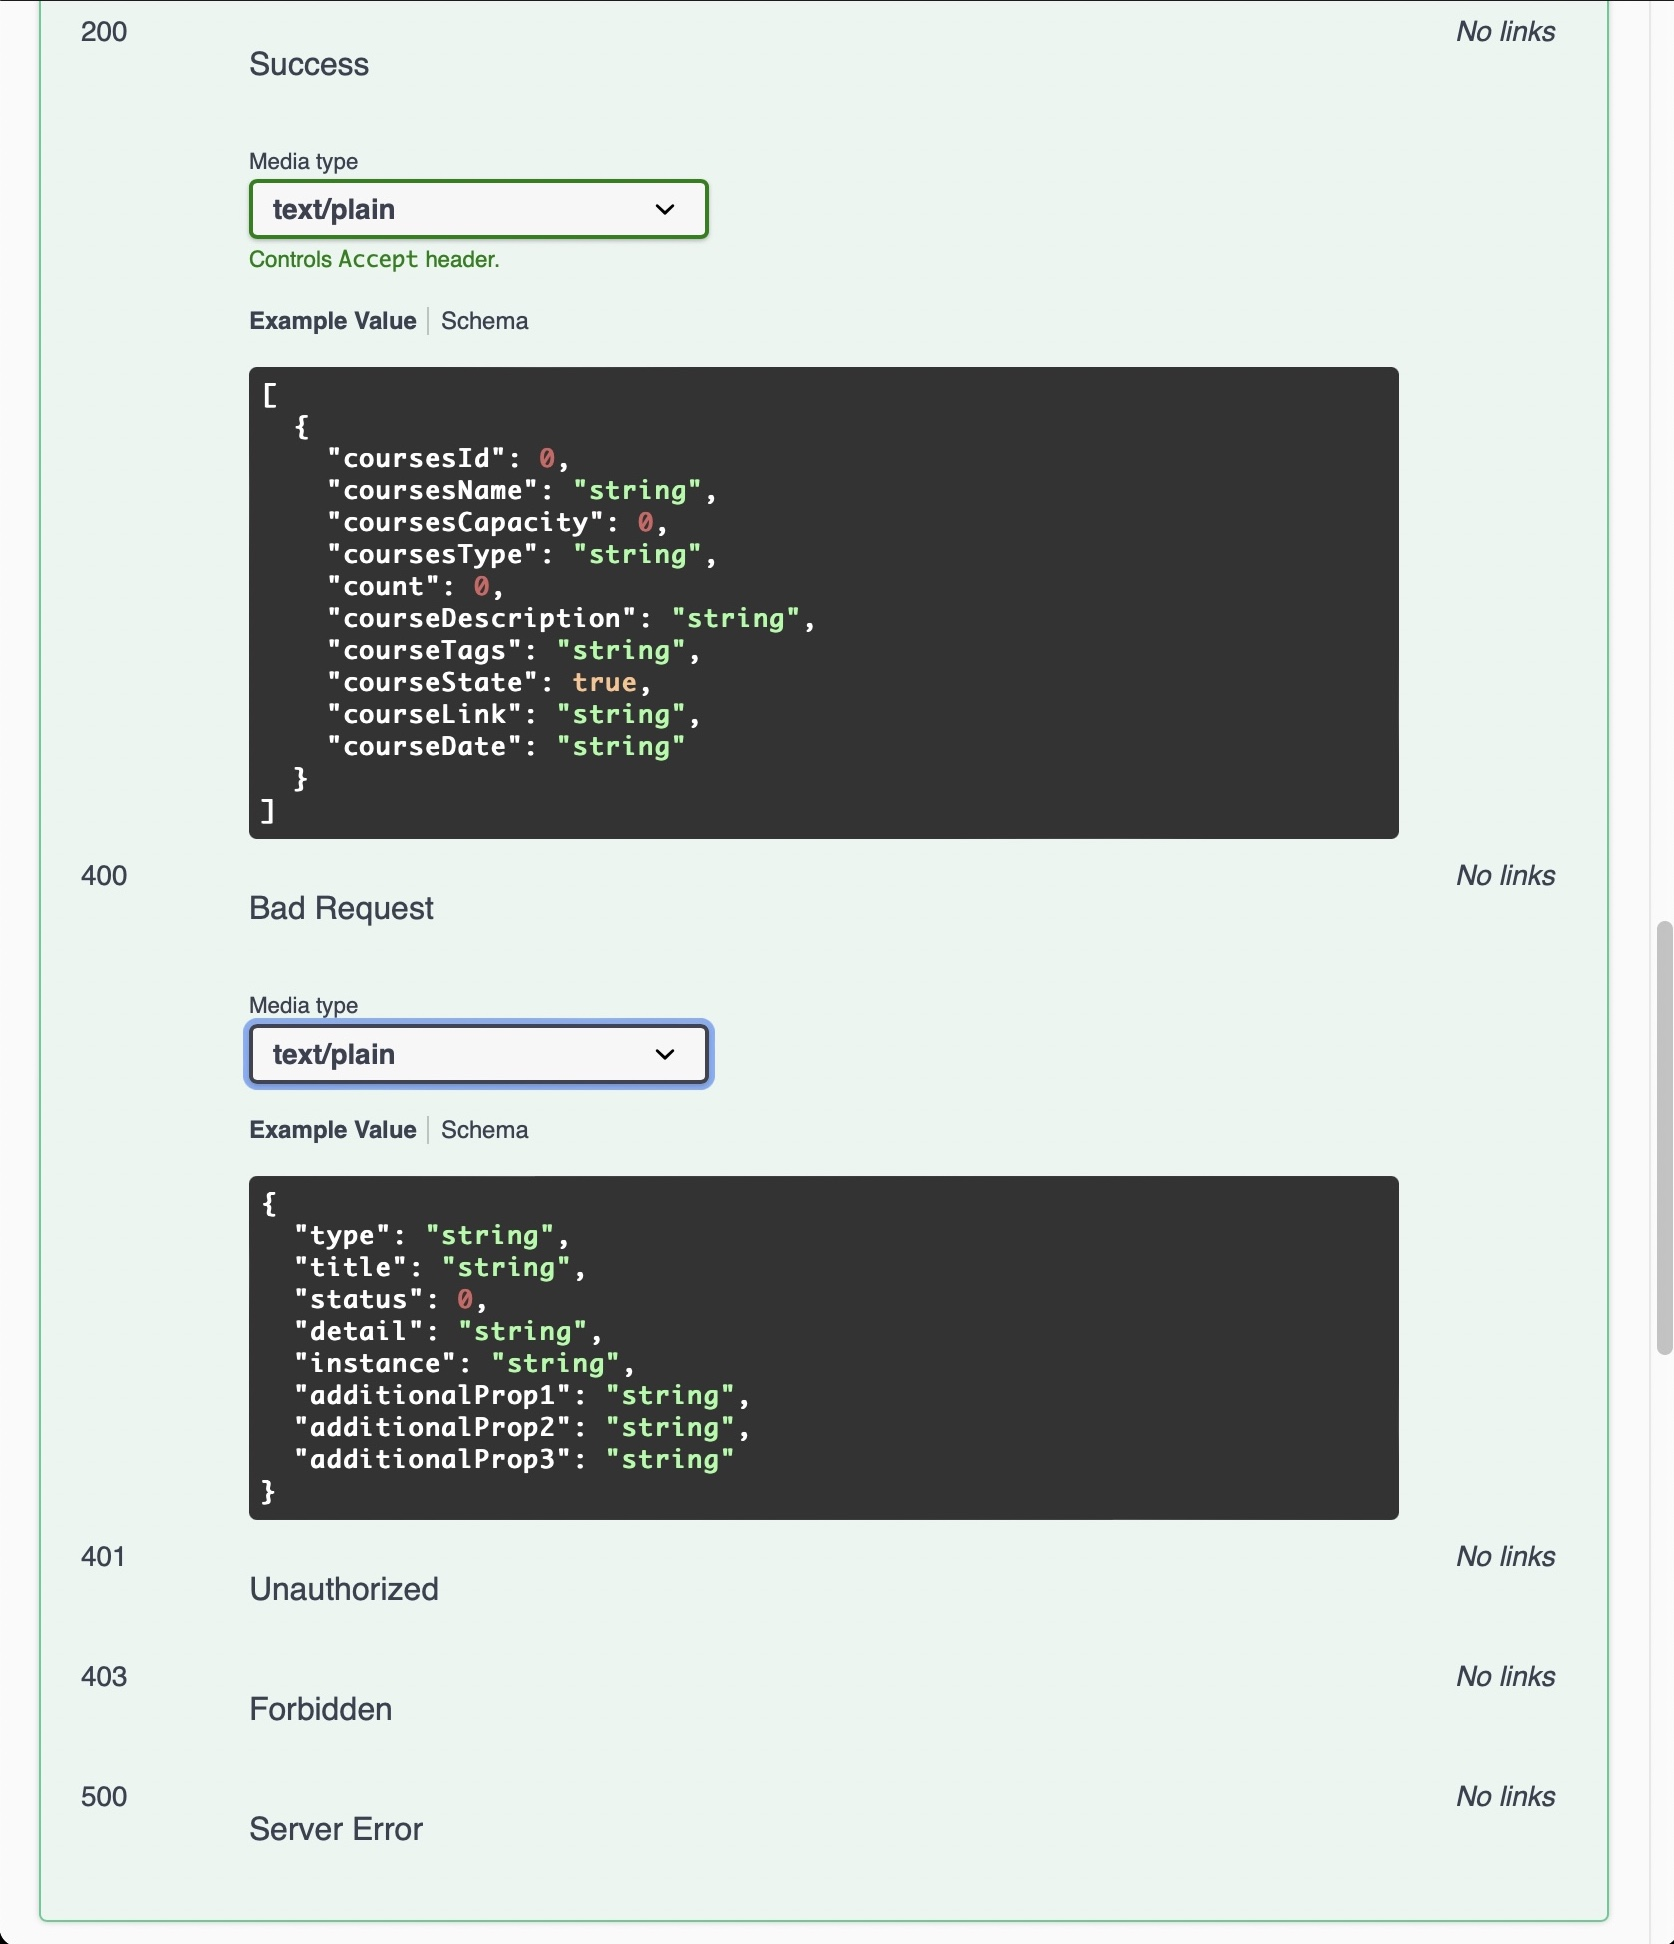
\includegraphics[width=1\textwidth]{Images/swagger success.jpg}
\caption{\label{fig:swagger success}Alcuuni esempi di risultati di esecuzione di \acrshort{api} tramite Swagger, in ordine \texttt{200, Successo}, \texttt{400, `Cattiva richiesta'}, \texttt{401, `Non autorizzato'}, \texttt{403, `Vietato'} e \texttt{500, `Errore interno del server'}.}
\end{figure}


% frontend %%%%%%%%%%%%%%%%%%%%%%%%%%%%%%%%%%%%%%%%%%%%%%%%%%%%%%%%%%%%%%%%%%%%%%%%%%%%%%%%%%%%%%%%%%%%%%%%%%
\newpage
\section{Frontend}\label{sec:frontend}
Questa sezione descriverà come ho usato Angular per lo sviluppo e la ratio dietro le scelte progettuali riguardanti il livello di presentazione del progetto di prova finale, ossia il frontend.\newline

L'unico requisito di sistema è stato avere \acrfull{npm} installato, in quanto Angular è un framework che si basa su di esso.
\acrshort{npm} è un gestore di pacchetti per \acrshort{js}, in particolare è quello di default per Node.js, un ambiente d'esecuzione \acrshort{js}.
\acrshort{npm} è composto da un client da linea di comando e un database online di pacchetti pubblici e privati, chiamato \acrfull{npm} registry. 
Per installare \acrshort{npm} più agevolemnte, ho usato \acrfull{nvm}, un gestore di versioni di Node.js, il quale permette di installare e gestire più versioni di Node.js su un sistema. Di seguito, il codice bash per installare \acrshort{nvm}: 
\begin{lstlisting}[language=bash, linewidth=20cm, basicstyle=\tiny]
curl -o- https://raw.githubusercontent.com/nvm-sh/nvm/v0.39.0/   install.sh | bash
\end{lstlisting}

Una volta fatto ciò, è stato necessario installare la versione 16 di Node.js, la quale è stata usata per lo sviluppo del frontend. Di seguito, il codice bash per installare la versione 16 di Node.js:
\begin{lstlisting}[language=bash, linewidth=20cm, basicstyle=\tiny]
nvm install 16
nvm use 16.x.x
\end{lstlisting}

Il passo successivo è stato quello di installare tutte le dipendenze necessarie per far funzionare il frontend del progetto di prova finale. Di seguito, il relativo codice da eseguire su terminale:
\begin{lstlisting}[language=bash, linewidth=20cm, basicstyle=\tiny]
npm install #(npm v 16.18.1)
\end{lstlisting}

Infine, è stato necessario compilare e avviare il frontend. Di seguito, il relativo codice da eseguire su terminale:
\begin{lstlisting}[language=bash, linewidth=20cm, basicstyle=\tiny]
npm run build #l'equivalente di `ng build'
npm run start #l'equivalente di `ng serve'
\end{lstlisting}

Finalmente, è stato possibile accedere all'interfaccia grafica (\acrshort{gui}) del frontend, digitando e navigando all'indirizzo \texttt{http://localhost:4200/} su un qualsiasi browser.
\textbf{Nota che } le scritte in verde, precedute da un `\#', sono commenti, quindi non vengono eseguite dal terminale.\newline

Passando allo sviluppo del codice vero e proprio, ho utilizzato la \acrshort{cli} di Angular, la quale mi ha permesso di creare nuovi componenti, direttamente da terminale, con un solo comando. Il codice bash per installarla è:
\begin{lstlisting}[language=bash, linewidth=20cm, basicstyle=\tiny]
npm install -g @angular/cli
\end{lstlisting}

Di seguito, il codice bash per creare un nuovo componente:
\begin{lstlisting}[language=bash, linewidth=20cm, basicstyle=\tiny]
ng generate component education #crea un nuovo componente chiamato `educationComponent', per gestire i corsi formativi, dal punto di vista di un utente base
\end{lstlisting}

Se il comando viene eseguito correttamente, verrà creato una nuova cartella, chiamata \texttt{education}, all'interno della cartella \texttt{src/app/components}, con i file necessari per far funzionare il componente, come si può vedere dalla figura (\ref{fig:education}).
\begin{figure}[H]
\centering
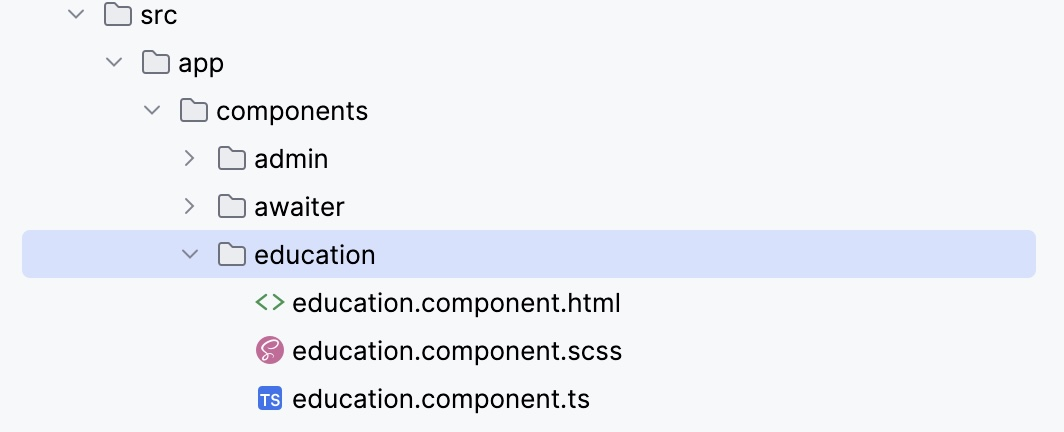
\includegraphics[width=1\textwidth]{Images/education.jpg}
\caption{\label{fig:education}La struttura della cartella \texttt{education}, creata tramite la \acrshort{cli} di Angular.}
\end{figure}

Una volta creato il componente, è stato necessario configurare il file che si occupa di gestire l'instradamento dell'applicazione, \texttt{app-routing.module.ts}, per poter visualizzare correttamente il nuovo componente. Successivamente è stato necessario configurare il file \texttt{app.module.ts}: in particolare, è stato necessario importare il nuovo componente e aggiungerlo all'array \texttt{declarations} del modulo \texttt{NgModule}. Di seguito, il codice in TypeScript del file \texttt{app.module.ts} e del file \texttt{app-routing.module.ts}:
\begin{figure}[H]
\centering
\begin{lstlisting}[language=TypeScript, linewidth=20cm, basicstyle=\tiny]
import {EducationManagementComponentComponent} from './components/admin/educationManagementComponent/ educationManagementComponent.component';
import {EducationComponent} from './components/education/  education.component';
import {CoursesEffect} from "./redux/courses/courses.effects";
import {CoursesResolver} from "./resolvers/courses.resolver";
import {EnrollmentComponent} from "./components/enrollment/enrollment.component";
\end{lstlisting}
\caption{\label{fig:app.module import}Tutti i componenti e i servizi importati nel file \texttt{app.module.ts}, anche quelli che verranno descritti successivamente.}
\end{figure}

\begin{figure}[H]
\centering
\begin{lstlisting}[language=TypeScript, linewidth=20cm, basicstyle=\tiny]
@NgModule({
  bootstrap: [AppComponent],
  declarations: [
  AppComponent,
  AwaiterComponent,
  MessageComponent,
  AppMainComponent,
  AppConfigComponent,
  AppLoginComponent,
  AppNotfoundComponent,
  AppErrorComponent,
  AppAccessdeniedComponent,
  DurationPipe,

  NoticeComponent,
  ReservationComponent,
  OfficesManagementComponent,
  NoticesManagementComponent,
  ViewsManagementComponent,

  EducationManagementComponentComponent,
  EducationComponent,
  EnrollmentComponent,
  ],
  imports: [
  ...
  ],
  providers: [
  ...
  ]
})
export class AppModule {}
\end{lstlisting}
\caption{\label{fig:app.module ngmodule}L'array \texttt{declarations} del modulo \texttt{NgModule} del file \texttt{app.module.ts}, con l'aggiunta dei componenti sviluppati per il progetto di prova finale.}
\end{figure}
\textbf{Nota che } i puntini rappresentano l'omissione di codice non rilevante ai fini della spiegazione.\newline

\begin{figure}[H]
\centering
\begin{lstlisting}[language=TypeScript, linewidth=20cm, basicstyle=\tiny]
import ...
import { EnrollmentComponent } from "./components/enrollment/enrollment.component";
import { EducationComponent } from "./components/education/education.component";
import { EducationManagementComponentComponent } from "./components/admin/educationManagementComponent/  educationManagementComponent.component";

@NgModule({
  imports: [ RouterModule.forRoot([
    { path: "", redirectTo: "/notice", pathMatch: "full" },
    {
     path: "",
     component: AppLayoutComponent,
     children: [ { ... }
      {
       path: "education",
       component: EducationComponent,
       canActivate: [GuestUserGuard, BaseUserGuard, VipUserGuard, AdminUserGuard],
       resolve: { coursesData: "CoursesResolver"},
      },
      {
       path: "educationManagementComponent",
       component: EducationManagementComponentComponent,
       canActivate: [AdminUserGuard],
       resolve: { coursesData: "CoursesResolver"},
      }
     ],
    },
    { path: "error", component: AppErrorComponent },
    { path: "access", component: AppAccessdeniedComponent },
    { path: "notfound", component: AppNotfoundComponent },
    { path: "login", component: AppLoginComponent },
   ],
   { scrollPositionRestoration: "enabled" }
  ),],
  exports: [RouterModule],
  providers: [GuestUserGuard, BaseUserGuard, VipUserGuard,   AdminUserGuard],
})
export class AppRoutingModule {}
\end{lstlisting}
\caption{\label{fig:app.routing}Il codice del file \texttt{app-routing.module.ts}, il quale si occupa di instradare l'applicazione, a seconda dell'utente e della `guardia' attivata.}
\end{figure}
\textbf{Nota che } i puntini rappresentano l'omissione di codice non rilevante ai fini della spiegazione.\newline

Una volta che il componente è stato configurato correttamente all'interno dei file sopra citati, è stato possibile iniziare a sviluppare il codice del componente stesso. Ossia i file:
\begin{itemize}
  \item \texttt{education.component.html}, il quale si occupa di gestire la parte \acrshort{html} del componente, è quindi il template dello stesso;
  \item \texttt{education.component.ts}, il quale si occupa di gestire la parte TypeScript del componente;
\end{itemize}
\textbf{Nota che } il file \texttt{education.component.css} è stato omesso, in quanto vuoto, perchè il \acrshort{css} di ogni componente è stato gestito tramite il file \texttt{styles.css}, come si può notare dalla figura (\ref{fig:styles}).\newline

\begin{figure}[H]
\centering
\begin{lstlisting}[language=HTML, linewidth=20cm, basicstyle=\tiny]
<div class="card">
   <div class="flex"> <span style="font-size: 25px;">Gestione corsi (Admin)</span> </div>
   <div class="container mt-5">
      <h4 class="mb-4">{{ showAddForm ? 'Aggiungi' : 'Modifica' }} corso</h4>
      <form (ngSubmit)="showAddForm ? addCourse(courseForm) : updateCoursesData(courseForm)" #courseForm="ngForm">
        <div class="p-grid">
           <div class="p-col-12 p-md-6">
              <div class="p-inputgroup">
                <span class="p-float-label">
                   <input *ngIf="showAddForm" pInputText name="name" [(ngModel)]="course.coursesName" required>
                   <input *ngIf="!showAddForm" pInputText name="name" [(ngModel)]="editedCourse.coursesName" required> <label>Nome corso</label>
                </span>
              </div>
              <ng-container *ngIf="courseForm.controls['name']">
                <ng-container *ngIf="courseForm.controls['name'].invalid && (courseForm.controls['name'].dirty || courseForm.controls['name']        .touched)">
                   <div class="error-message" *ngIf="courseForm.controls['name'].errors.required">
                      Nome corso obbligatorio
                   </div>
                </ng-container>
              </ng-container>
           </div>
           <br>
           <div class="p-col-12 p-md-6">
              <div class="p-inputgroup">
                <span class="p-float-label">
                   <input *ngIf="showAddForm" pInputText name="capacity" [(ngModel)]="course.coursesCapacity" required>
                   <input *ngIf="!showAddForm" pInputText name="capacity" [(ngModel)]="editedCourse.coursesCapacity" required> <label>Numero postazioni</label>
                </span>
              </div>
              <ng-container *ngIf="courseForm.controls['capacity']">
                <ng-container *ngIf="courseForm.controls['capacity'].invalid && (courseForm.controls['capacity'].dirty || courseForm.controls['capacity'].touched)">
                   <div class="error-message" *ngIf="courseForm.controls['capacity'] .errors.required">
                      Numero postazioni obbligatorio
                   </div>
                </ng-container>
              </ng-container>
           </div>
           <br>
           <div class="p-col-12">
              <div class="p-inputgroup">
                <span class="p-float-label ">
                   <p-dropdown *ngIf="showAddForm" [options]="types" [(ngModel)]="selectedType" placeholder="Seleziona tiopologia corso"              optionLabel = "types" name="types" [style]="{ 'width': '100%' }" required></p-dropdown>
                   <p-dropdown *ngIf="!showAddForm" [options]="types" [(ngModel)]="selectedType" placeholder="Seleziona tiopologia corso"  optionLabel="types" name="types" [style]="{ 'width': '100%' }" required></p-dropdown> <label>Seleziona tipologia corso     </label>
                </span>
              </div>
              <ng-container *ngIf="courseForm.controls['coursesType']">
                <ng-container *ngIf="courseForm.controls['coursesType'].invalid && (courseForm.controls['coursesType'].dirty || courseForm.controls['coursesType'].touched)">
                   <div class="error-message" *ngIf="courseForm.controls['coursesType'] .errors.required">
                      Tipologia corso obbligatoria
                   </div>
                </ng-container>
              </ng-container>
           </div>
        </div>
        <br>
        <div class="p-col-12 p-md-6">
           <div class="p-inputgroup">
              <span class="p-float-label">
                <p-calendar *ngIf="showAddForm" [(ngModel)]="course.coursesDate" name="date" dataType="string" dateFormat="dd/mm/yy" [showIcon] = "      true" required> </p-calendar>
                <p-calendar *ngIf="!showAddForm" [(ngModel)]="editedCourse.coursesDate" name="date" dataType="string" dateFormat="dd/mm/yy" [  showIcon]="true" required></p-calendar> <label>Data inizio corso </label>
              </span>
           </div>
           <ng-container *ngIf="courseForm.controls['coursesDate']">
              <ng-container *ngIf="courseForm.controls['coursesDate'].invalid && (courseForm.controls['coursesDate'].dirty || courseForm.controls['coursesDate'].touched)">
                <div class="error-message" *ngIf="courseForm.controls['coursesDate'] .errors.required">
                   Data inizio obbligatoria
                </div>
              </ng-container>
           </ng-container>
        </div><br><br><br>
        <div *ngIf="showAddForm">
           <button pButton type="submit" label="Aggiungi corso" class="p-button-rounded p-button-success" [disabled]="courseForm.invalid || selectedUsers.length > course.coursesCapacity"></button>
           <div *ngIf="successAdd" class="success-message">
              Corso aggiunto correttamente!
           </div>
           <div class="error-message" *ngIf="selectedUsers.length > course.coursesCapacity">
              Il numero di utenti inseriti supera la disponibilita' del corso
           </div>
        </div>
       ...
\end{lstlisting}
\caption{\label{fig:education form}Il codice \acrshort{html} del file \texttt{education.component.html}, in particolare il form per l'aggiunta e la modifica dei corsi di formazione.}
\end{figure}
\textbf{Notiamo che } una parte del codice è stata omessa, tramite dei puntini, in quanto identica al `div' precedente, ma invece di gestire l'aggiunta dei corsi, ne gestisce la modifica.\newline

Analizzando il codice soprastante (\ref{fig:education form}), la parte del template \acrshort{html} contenente la totalità dei \texttt{div} che compongono il form\footnote{\glsdesc{form}} per la gestione dei corsi di formazione -da parte dell'admin- troviamo tre azioni principali disponibili:
\begin{itemize}
  \item \texttt{addCourse}, il quale raccoglie i dati inseriti dall'utente tramite un form apposito e i container di \acrshort{primeng} -i quali verranno trattati più approfonditamente nella sezione (\ref{subsec:primeng})- e li invia al backend, tramite i metodi \acrshort{ts} appositi;
  \item \texttt{updateCoursesData}, il quale condivide il form d'inserimento dati con \texttt{addCourse}, ma solamente dopo che l'utente ha cliccato il pulsante di modifica apposito, nella tabella dei corsi di formazione. Ovviamente, invierà comunque i dati al backend, ma stavolta per aggiornare una tupla già esistente;
  \item \texttt{deleteCoursesData}, il quale si occupa di cancellare una tupla, e quindi un corso, già esistente, tramite il metodo \acrshort{ts} apposito e una semplice query.
\end{itemize}
Inoltre, ogni campo del form è dotato degli appositi attrubuti \texttt{required}, per garantire che l'utente non possa inviare un form vuoto, e \texttt{ngModel}, per legare i dati inseriti dall'utente al componente \acrshort{ts} corrispondente e ogni azione è accompagnata da un messaggio di successo o di errore, il quale verrà mostrato all'utente, tramite un \texttt{div} apposito, in caso di esito positivo o negativo.\newline

\begin{figure}[H]
\centering
\begin{lstlisting}[language=HTML, linewidth=20cm, basicstyle=\tiny]
<p-table styleClass="p-datatable-courses-data" [value]="coursesData$ | async" dataKey="chargePointId"
currentPageReportTemplate="Showing {first} to {last} of {totalRecords} entries" responsiveLayout="scroll"
[rows]="5" [rowHover]="true" [paginator]="true" [showCurrentPageReport]="true" [rowsPerPageOptions]="[5,10,15]"
[loading]="isLoading$ | async" [totalRecords]="totalRecords$ | async" [filterDelay]="300"
[globalFilterFields]="globalFiltersFields" [(selection)]="selectedCoursesData" [lazy]="true" [customSort]="true"
(onLazyLoad)="sort($event)" [tableStyle]="{'min-width': '25rem'}">
    <ng-template pTemplate="caption">
        <div class="flex">
            <span style="font-size: 25px;">Elenco corsi creati</span>
            <span class="p-input-icon-left ml-auto">
                <i class="pi pi-search"></i>
                <input pInputText [value]="lastSearch$ | async" type="text" (input)="filter($event.target.value)" placeholder="Course Search" />
            </span>
        </div>
    </ng-template>
    <ng-template pTemplate="header">
        <tr>
            <th pSortableColumn="coursesName">
                <div class="p-d-flex p-jc-between p-ai-center">
                    Nome corso
                    <p-sortIcon field="coursesName"></p-sortIcon>
                </div>
            </th>
            <th>
                <div class="p-d-flex p-jc-between p-ai-center">
                    Partecipanti max
                </div>
            </th>
            <th pSortableColumn="coursesType">
                <div class="p-d-flex p-jc-between p-ai-center">
                    Tipologia
                    <p-sortIcon field="coursesType"></p-sortIcon>
                </div>
            </th>
            <th pSortableColumn="coursesDate">
                <div class="p-d-flex p-jc-between p-ai-center">
                    Data inizio
                    <p-sortIcon field="coursesDate"></p-sortIcon>
                </div>
            <th>
                <div class="p-d-flex p-jc-between p-ai-center">
                    Modifica
                </div>
            </th>
            <th>
                <div class="p-d-flex p-jc-between p-ai-center">
                    Elimina
                </div>
            </th>
        </tr>
    </ng-template>
    <ng-template pTemplate="body" let-coursesData>
        <tr class="p-selectable-row" [pRowToggler]="coursesData.coursesId">
            <td>
                <span class="p-column-title">Nome corso</span>
                {{coursesData.coursesName}}
            </td>
            <td>
                <span class="p-column-title">Num. postazioni max</span>
                {{coursesData.coursesCapacity}}
            </td>
            <td>
                <span class="p-column-title">Tipologia</span>
                {{coursesData.coursesType}}
            </td>
            <td>
                <span class="p-column-title">Data inizio</span>
                {{coursesData.coursesDate}}
            </td>
            <td>
                <span class="p-column-title">Modifica</span>
                <p-button icon="pi pi-file-edit" (click)="editCoursesData(coursesData); showAddForm = false;"></p-button>
            </td>
            <td>
                <span class="p-column-title">Elimina</span>
                <p-button icon="pi pi-trash" (click)='deleteCoursesData(coursesData)'></p-button>
            </td>
        </tr>
    </ng-template>
    <ng-template pTemplate="emptymessage">
        <tr>
            <td colspan="9">No Courses Data found.</td>
        </tr>
    </ng-template>
</p-table>
\end{lstlisting}
\caption{\label{fig:education table}Il codice \acrshort{html} del file \texttt{education.component.html}, in particolare la tabella per la visualizzazione dei corsi di formazione, coi relativi pulsanti per la modifica e la cancellazione.}
\end{figure}
\textbf{Notiamo che } in entrambe le figure (\ref{fig:education form}) e (\ref{fig:education table}), il codice \acrshort{html} è complementato da alcuni tag di \acrshort{primeng} -come \texttt{p-inputText}, \texttt{p-dropdown}, \texttt{p-calendar}, \texttt{p-table}, \texttt{p-sortableColumn}, \texttt{p-sortIcon}, \texttt{p-button}-, ma ne parleremo più approfonditamente nella sezione (\ref{subsec:primeng}).\newline

Al fine di creare la tabella per la visualizzazione dei corsi di formazione esistenti, ho utilizzato il componente \texttt{p-table} di \acrshort{primeng}, in modo da visualizzare correttamente i dati dei corsi provenienti dal backend. In particolare, il template \acrshort{html} è strettamente legato ai tag \texttt{ng-template}, i quali permettono di definire un template personalizzato per la visualizzazione dei dati, in base alle esigenze dello sviluppatore. Così facendo, risulta il codice di una tabella \acrshort{html} classica, ma potenziata da \acrshort{primeng} e che comunica correttamente con il livello della logica di business.
Un'altra funzionalità offerta da \acrshort{primeng} e usata nel codice soprastante è la possibilità di ordinare i dati della tabella, tramite il tag \texttt{p-sortableColumn} e \texttt{p-sortIcon}, i quali permettono di ordinare i dati in base a una colonna, in ordine crescente o decrescente, e di visualizzare la relativa icona che indica l'ordine corrente.\newline 

\begin{figure}[H]
\centering
\begin{lstlisting}[language=TypeScript, linewidth=20cm, basicstyle=\tiny]
import ...
import { CoursesData } from 'src/app/redux/courses/courses.state';
import { selectCoursesData, selectCoursesDataFilters } from 'src/app/redux/courses/courses.selectors';
import { addCoursesData, changeCoursesDataFilters, deleteCoursesData, updateCoursesData } from 'src/app/redux/courses/courses.actions';
@Component({
    selector: 'app-educationManagementComponent',
    templateUrl: './educationManagementComponent.component.html',
    styleUrls: ['./educationManagementComponent.component.scss'],
})
export class EducationManagementComponentComponent  implements OnInit, OnDestroy{
    coursesData$: Observable<CoursesData[]> = of([]);
    public editedCourse: Partial<CoursesData> = {};
    course: Partial<CoursesData> = { coursesName : '', coursesCapacity : null, coursesType: '', coursesDate: '' };
    types: any = [ { types: 'Udemy' }, { types: 'Coursera' }, { types: 'brilliant' }, { types: 'UniGe' }, { types: 'Angular University' } ];
    selectedType: any = null;
    usersId: any[] = [ { usersId: 'Utente 1' }, { usersId: 'Utente 2' }, { usersId: 'Utente 3' }, ];
    selectedUsers: any[] = [];
    showAddForm = true;
    successAdd = false;
    successUpdate = false;
    expandedMap: { [key: number]: boolean } = {};
    lastSearch$: Observable<string> = of(null);
    coursesDataFilters$: Observable<DynamicQueryPart> = of({});
    isLoading$: Observable<boolean>;
    totalRecords$: Observable<number> = of(0);
    globalFiltersFields = Object.keys(this.course);
    filtersSubj$ = new Subject<Action>();
    filtersSub: Subscription;
    private firstQuery = true;
    private _selectedCoursesData: CoursesData;
    get selectedCoursesData() { return this._selectedCoursesData; }
    set selectedCoursesData(value: CoursesData) { this._selectedCoursesData = value; }
    constructor(
        private store: Store<AppState>,
        private route: ActivatedRoute
    ){
        this.coursesData$.subscribe((data) => {
            if (data) { data.forEach((course) => {this.expandedMap[course.coursesId] = false; }); } });
        this.isLoading$ = store.select(selectIsLoading).pipe(distinctUntilChanged());
        this.coursesDataFilters$ = store.select(selectCoursesDataFilters);
        this.filtersSub = this.filtersSubj$.asObservable().pipe(debounceTime(1000)).subscribe((a) => this.store.dispatch(a));
        this.lastSearch$ = store.select(selectCoursesDataFilters).pipe(take(1), map((f) => f.filtering && f.filtering.length > 0 ? f.filtering[0]        .value : ''));
    }
    addCourse(form: NgForm) {
        if (this.selectedType) this.course.coursesType = this.selectedType.types;
        if (this.selectedUsers.length > 0) this.selectedUsers.map((user) => user.usersId);
        this.store.dispatch( addCoursesData({ item: this.course, _id: getRandomId() }) );
        this.resetFormFields(form);
        this.successAdd = true;
        this.successUpdate = false;
    }
    resetFormFields(form: NgForm) {
        form.resetForm();
        this.course = { coursesId: null, coursesName: '', coursesCapacity : null, coursesDate: null };
        this.selectedType = null;
        this.selectedUsers = [];
    }
    deleteCoursesData(course: CoursesData){ if (course) this.store.dispatch( deleteCoursesData({item: course, _id: getRandomId() })); }
    updateCoursesData(form: NgForm){
        if (this.selectedUsers.length > 0) this.selectedUsers.map((user) => user.usersId);
        if (this.selectedType) this.editedCourse.coursesType = this.selectedType.types;
        this.store.dispatch( updateCoursesData({ item: this.editedCourse , _id: getRandomId() }) );
        this.editedCourse = {};
        this.resetFormFields(form);
        this.successUpdate = true;
        this.successAdd = false;
        this.showAddForm = true;
    }
    editCoursesData(course: CoursesData) {
        this.editedCourse  = { ...course };
        this.showAddForm = false;
    }
    async filter(value: string) {
      ... //vedi figura successiva
    }
    async sort($event: LazyLoadEvent) {
        ... //vedi figura successiva
    }
    ngOnInit(): void {
        this.coursesData$ = this.store.select(selectCoursesData).pipe(startWith(this.route.snapshot.data.CoursesData));
        this.coursesData$.pipe(
            filter(data => !!data)
        ).subscribe(() => {
            this.totalRecords$ = this.coursesData$.pipe(map((x) => (x ? (x[0] ? x[0].count : 0) : 0)));
        });
    }
    ngOnDestroy(): void { this.filtersSub?.unsubscribe(); }
}
\end{lstlisting}
\caption{\label{fig:education.ts}Il codice TypeScript del file \texttt{education.component.ts}.}
\end{figure}
\begin{figure}[H]
\centering
\begin{lstlisting}[language=TypeScript, linewidth=20cm, basicstyle=\tiny]
async filter(value: string) {
    const currentQueryParams = await firstValueFrom(this.coursesDataFilters$.pipe(take(1)));
    const newQueryParams: DynamicQueryPart = {
        ...currentQueryParams,
        paging: currentQueryParams.paging
            ? currentQueryParams.paging
            : { skip: 0, take: environment.defaultNumberOfRowsPerPage },
        filtering: value
            ? [{ column: this.globalFiltersFields.join(','), predicate: 'LK', value, kind: 'STRING' } as Filtering]
            : []
    };
    this.filtersSubj$.next(changeCoursesDataFilters({ queryParams: newQueryParams, _id: getRandomId() }));
}
async sort($event: LazyLoadEvent) {
    if (this.firstQuery) {
        this.firstQuery = false;
        return;
    }
    const currentQueryParams = await firstValueFrom(this.coursesDataFilters$.pipe(take(1)));
    const newQueryParams = {
        ...currentQueryParams,
        ordering: $event.sortField
            ? [{ column: $event.sortField, columnPrefix: '', descending: $event.sortOrder > 0}]
            : [],
        paging: currentQueryParams.paging
            ? ($event.first !== null || true)
                ? { skip: $event.first, take: $event.rows }
                : currentQueryParams.paging
            : { skip: 0, take: environment.defaultNumberOfRowsPerPage }
    };
    this.filtersSubj$.next(changeCoursesDataFilters({ queryParams: newQueryParams, _id: getRandomId() }));
}
\end{lstlisting}
\caption{\label{fig:sort and filter}I metodi \texttt{filter} e \texttt{sort} del file \texttt{education.component.ts}, i quali si occupano di filtrare e ordinare i corsi di formazione, listati qui per motivi di spazio rispetto alla figura precedente.}
\end{figure}

Come si può vedere dalle figure (\ref{fig:education.ts}) e (\ref{fig:sort and filter}), il componente \acrshort{ts} si occupa di gestire la totalità della logica di business del componente \texttt{educationComponent}, in particolare, le nozioni principali sono:
\begin{itemize}
  \item alcuni \texttt{import} sono stati omessi, in quanto non rilevanti ai fini della spiegazione;
  \item gli \texttt{import} alle righe 2, 3 e 4 sono relativi ai file e ai servizi necessari per far funzionare correttamente la logica di business del componente;
  \item il componente implementa l'interfaccia \texttt{OnInit} e \texttt{OnDestroy}, in modo da poter eseguire del codice all'inizializzazione e alla distruzione del componente;
  \item il componente è dotato di variabili, le quali si occupano di gestire la totalità dei dati e delle azioni del componente, come ad esempio \texttt{coursesData\$} e \texttt{course}, le quali si occupano rispettivamente di tenere in memoria un array dei corsi esistenti e di fissare i dati di un corso, in modo da poterla usare come puntatore per un ciclo di aggiunta o modifica di un corso;
  \item il metodo \texttt{addCourse} si occupa di raccogliere i dati del backend e iniettarli nel livello di presentazione;
  \item il metodo \texttt{resetFormFields} si occupa di resettare i campi del form, in modo da poter inserire nuovi dati;
  \item il metodo \texttt{deleteCoursesData} si occupa di cancellare un corso esistente, tramite il metodo \acrshort{ts} apposito e una semplice query;
  \item il metodo \texttt{filter} si occupa di filtrare i dati dei corsi di formazione;
  \item il metodo \texttt{sort} si occupa di ordinare i dati dei corsi di formazione ricevuti dal backend, per poterli visualizzare correttamente nella tabella del livello di presentazione.
\end{itemize}

\begin{figure}[H]
\centering
\begin{lstlisting}[language=CSS, linewidth=20cm, basicstyle=\tiny]
$gutter: 1rem; //for primeflex grid system

@import "assets/layout.scss";

@import "../node_modules/primeng/resources/primeng.min.css";
@import "../node_modules/primeflex/primeflex.scss";
@import "../node_modules/primeicons/primeicons.css";

@import "assets/overrides/styles/theme.scss";  
\end{lstlisting}
\caption{\label{fig:styles}Il codice \acrshort{css} del file \texttt{styles.css}, il quale si occupa di gestire il \acrshort{css} di tutti i componenti, importando temi e stili da \acrshort{primeng}.}
\end{figure}
In questo caso, il progetto, non concentrandosi sull'apprendimento del dettaglio di uno stile, ma sull'implementazione di un prototipo, ho deciso di usare un tema predefinito di \acrshort{primeng}, il quale è stato importato nel file \texttt{styles.css}, come si può vedere dalla figura (\ref{fig:styles}). Nonostante la leggera perdità di personalizzazione, la scelta di usare un tema predefinito ha permesso di efficientare i tempi di sviluppo, in quanto non è stato necessario scrivere \acrshort{css} da zero -spesso complicato-, ma solo importare un tema già pronto.\newline


TODO spiegazione di course.effects, course.actions, course.
reducers, course.state e course.selectors
ALtri file degni di nota sono:
\begin{itemize}
  \item \texttt{courses.actions.ts}, il quale contiene tutti gli \texttt{export} delle azioni relative ai corsi di formazione, come si vede dalla figura (\ref{fig:courses.actions});
  \item \texttt{courses.effects.ts}, il quale si occupa principalmente di mappare le informazioni in entrata o in uscita dal componente, come si vede dalla figura (\ref{fig:courses.effects});
  \item \texttt{courses.reducer.ts}, il quale contiene alcuni metodi ausiliari per il corretto funzionamento della logica di business, in particolare per filtrare o manipolare le informazioni dal o verso il backend, come si vede dalla figura (\ref{fig:courses.reducer});
  \item \texttt{courses.state.ts}, il quale contiene la struttura di base dello stato dei corsi di formazione, come si vede dalla figura (\ref{fig:courses.state});
  \item \texttt{courses.selectors.ts}, il quale gli \texttt{export} necessari per il funzionamento di ogni metodo filtro o di stato dei corsi di formazione, come si vede dalla figura (\ref{fig:courses.selectors}).
\end{itemize}

\begin{figure}[H]
\centering
\begin{lstlisting}[language=TypeScript, linewidth=20cm, basicstyle=\tiny]
import {createAction, props} from '@ngrx/store';
import {DynamicQueryPart, WithId} from '../state';
import {SuccessPayload, ErrorPayload} from '../message/message.actions';
import {CoursesData} from './courses.state';

export const searchCoursesData = createAction('[API] Search Courses Data', props<{queryParams: DynamicQueryPart} & WithId>());
export const searchCoursesDataSuccess = createAction('[API] Search Courses Data Success', props<SuccessPayload<{result: CoursesData[]}> & WithId>());
export const searchCoursesDataError = createAction('[API] Search Courses Data Error', props<ErrorPayload & WithId>());
export const changeCoursesDataFilters = createAction('[API] Change Courses Data Filters', props<{queryParams: DynamicQueryPart} & WithId>());

export const addCoursesData = createAction('[API] Add Courses Data', props<{item: Partial<CoursesData>} & WithId>());
export const addCoursesDataSuccess = createAction('[API] Add Courses Data Success', props<SuccessPayload<{result: CoursesData[]}> & WithId>());
export const addCoursesDataError = createAction('[API] Add Courses Data Error', props<ErrorPayload & WithId>());

export const deleteCoursesData = createAction('[API] Delete Courses Data', props<{item: Partial<CoursesData>} & WithId>());
export const deleteCoursesDataSuccess = createAction('[API] Delete Courses Data Success', props<SuccessPayload<{result: CoursesData[]}> & WithId>());
export const deleteCoursesDataError = createAction('[API] Delete Courses Data Error', props<ErrorPayload & WithId>());

export const updateCoursesData = createAction('[API] Update Courses Data', props<{ item: Partial<CoursesData> } & WithId>());
export const updateCoursesDataSuccess = createAction('[API] Update Courses Data Success', props<SuccessPayload<{result: CoursesData[]}> & WithId>());
export const updateCoursesDataError = createAction('[API] Update Courses Data Error', props<ErrorPayload & WithId>());
\end{lstlisting}
\caption{\label{fig:courses.actions}Il codice TypeScript del file \texttt{courses.actions.ts}.}
\end{figure}

\begin{figure}[H]
\centering
\begin{lstlisting}[language=TypeScript, linewidth=20cm, basicstyle=\tiny]
import { Injectable } from '@angular/core';
import { ofType, createEffect, Actions } from '@ngrx/effects';
import { map, mergeMap, catchError } from 'rxjs/operators';
import { CustomHttpClient } from '../../services/custom-http-client.service';
import { environment } from '../../../environments/environment';  //  src/environments/environment';
import { addCoursesData, addCoursesDataError, addCoursesDataSuccess, changeCoursesDataFilters, deleteCoursesData, deleteCoursesDataError, deleteCoursesDataSuccess, searchCoursesData, searchCoursesDataError, searchCoursesDataSuccess, updateCoursesData, updateCoursesDataError, updateCoursesDataSuccess,} from './courses.actions';
import { CoursesData } from './courses.state';
import { HttpErrorResponse } from '@angular/common/http';
import { of } from 'rxjs/internal/observable/of';

@Injectable()
export class CoursesEffect{

    constructor(
        private actions$: Actions,
        private httpClient: CustomHttpClient
    ){ }

    _serachCoursesData = createEffect(
        () => this.actions$.pipe(
            ofType(searchCoursesData),
            mergeMap(a => {
                const response$ = this.httpClient.post<CoursesData[]>(`${environment.apiUrl}/courses/searchCoursesData`, a.queryParams, { responseType: 'json'});
                return response$.pipe(
                    map(r => r ?? []),
                    map(r => searchCoursesDataSuccess({result: r, _id: a._id })),
                    catchError((err: HttpErrorResponse, _) => {
                        return [searchCoursesDataError({error: err.message, _id: a._id})];
                    }));
            }))
    );

    _changeCoursesDataFilters = createEffect(
        () => this.actions$.pipe(
            ofType(changeCoursesDataFilters),
            map(a => searchCoursesData({queryParams: a.queryParams, _id: a._id}))
            )
    );

    _addCoursesData = createEffect(
        () => this.actions$.pipe(
            ofType(addCoursesData),
            mergeMap(a => {
                const response$ = this.httpClient.post<CoursesData[]>(`${environment.apiUrl}/courses/addCoursesData`, [a.item], { responseType: 'json'});
                return response$.pipe(
                    map(r => r ?? []),
                    map(r => addCoursesDataSuccess({result: r, _id: a._id })),
                    catchError((err: HttpErrorResponse, _) => {
                        return [addCoursesDataError({error: err.message, _id: a._id})];
                    }));
            }))
    );

    _deleteCoursesData = createEffect(
        () => this.actions$.pipe(
            ofType(deleteCoursesData),
            mergeMap(a => {
                const response$ = this.httpClient.delete<CoursesData[]>(`${environment.apiUrl}/courses/deleteCoursesData/${a.item.coursesId}` , { responseType: ' json'});
                return response$.pipe(
                    map(r => r ?? []),
                    map(r => deleteCoursesDataSuccess({result: r, _id: a._id })),
                    catchError((err: HttpErrorResponse, _) => {
                        return [deleteCoursesDataError({error: err.message, _id: a._id})];
                    }));
            }))
    );

    _updateCoursesData = createEffect(() =>
        this.actions$.pipe(
            ofType(updateCoursesData),
            mergeMap(a => 
                this.httpClient.put<CoursesData[]>(`${environment.apiUrl}/courses/updateCoursesData`, [a.item], { responseType: 'json' }
                ).pipe(
                    map(r => r ?? []),
                    map(r => updateCoursesDataSuccess({ result: r, _id: a._id })),
                    catchError((err: HttpErrorResponse, _) =>
                        of(updateCoursesDataError({ error: err.message, _id: a._id }))
                    )
                )
            )
        )
    );
}
\end{lstlisting}
\caption{\label{fig:courses.effects}Il codice TypeScript del file \texttt{courses.effects.ts}.}
\end{figure}

\begin{figure}[H]
\centering
\begin{lstlisting}[language=TypeScript, linewidth=20cm, basicstyle=\tiny]
import { createReducer, on, Action } from "@ngrx/store";
import { CoursesData, initialCoursesDataState as initialCoursesDataState, initialCoursesDataFiltersState as initialCoursesDataFiltersState } from "./courses.state";
import { DynamicQueryPart, WithId } from "../state";
import { addCoursesDataError, addCoursesDataSuccess, changeCoursesDataFilters, deleteCoursesDataError, deleteCoursesDataSuccess, searchCoursesDataError, searchCoursesDataSuccess, updateCoursesDataError, updateCoursesDataSuccess } from "./courses.actions";

const _coursesDataFiltersReducer = createReducer(
    initialCoursesDataFiltersState,
    on(changeCoursesDataFilters, (_, a) => ({...a.queryParams, _id: a._id}))
);
export function coursesDataFiltersReducer(state: DynamicQueryPart & WithId, action: Action): DynamicQueryPart & WithId{
    return _coursesDataFiltersReducer(state, action);
}

const  _coursesDataReducer = createReducer(
    initialCoursesDataState,
    on(searchCoursesDataSuccess, (_, a) =>
        Object.assign([...a.result ? a.result : []], { _id: a._id})),
    on(searchCoursesDataError, (_1, a) => Object.assign([], {_id: a._id})),
  );

export function coursesDataReducer(state: CoursesData[] & WithId, action: Action): CoursesData[] & WithId{
    return _coursesDataReducer(state, action);
}

const  _addCoursesDataReducer = createReducer(
    initialCoursesDataState,
    on(addCoursesDataSuccess, (_, a) =>
        Object.assign([...a.result ? a.result : []], { _id: a._id})),
    on(addCoursesDataError, (_1, a) => Object.assign([], {_id: a._id})),
  );

export function addCoursesDataReducer(state: CoursesData[] & WithId, action: Action): CoursesData[] & WithId{
    return _addCoursesDataReducer(state, action);
}

const  _deleteCoursesDataReducer = createReducer(
    initialCoursesDataState,
    on(deleteCoursesDataSuccess, (_, a) =>
        Object.assign([...a.result ? a.result : []], { _id: a._id})),
    on(deleteCoursesDataError, (_1, a) => Object.assign([], {_id: a._id})),
);

export function deleteCoursesDataReducer(state: CoursesData[] & WithId, action: Action): CoursesData[] & WithId{
    return _deleteCoursesDataReducer(state, action);
}

const  _updateCoursesDataReducer = createReducer(
    initialCoursesDataState,
    on(updateCoursesDataSuccess, (state, action) => ({ ...state, _id: action._id, coursesData: action.result })),
    on(updateCoursesDataError, (state, action) => ({ ...state, _id: action._id, error: action.error }))
);

export function updateCoursesDataReducer(state: CoursesData[] & WithId, action: Action): CoursesData[] & WithId{
    return _updateCoursesDataReducer(state, action);
}
  
\end{lstlisting}
\caption{\label{fig:courses.reducer}Il codice TypeScript del file \texttt{courses.reducer.ts}.}
\end{figure}

\begin{figure}[H]
\centering
\begin{lstlisting}[language=TypeScript, linewidth=20cm, basicstyle=\tiny]
import { DynamicQueryPart, WithId } from "../state";

export interface CoursesData {
    coursesId: number;
    coursesName: string;
    coursesCapacity: number;
    coursesType: string;
    coursesDate: string;
    count: number;
}

export const initialCoursesDataState: CoursesData[] & WithId = Object.assign([], {_id: ''});

export const initialCoursesDataFiltersState: DynamicQueryPart & WithId = {_id: ''};
\end{lstlisting}
\caption{\label{fig:courses.state}Il codice TypeScript del file \texttt{courses.state.ts}.}
\end{figure}

\begin{figure}[H]
\centering
\begin{lstlisting}[language=TypeScript, linewidth=20cm, basicstyle=\tiny]
import { createFeatureSelector, createSelector } from "@ngrx/store";
import { DynamicQueryPart, WithId } from "../state";
import { CoursesData } from "./courses.state";

export const selectCoursesDataState = createFeatureSelector<CoursesData[]>('coursesData');
export const selectCoursesDataFiltersState = createFeatureSelector<DynamicQueryPart>('coursesDataFilters');

export const selectCoursesData = createSelector(selectCoursesDataState, (state: CoursesData[] & WithId) => state);
export const selectCoursesDataFilters = createSelector(selectCoursesDataFiltersState, (state: DynamicQueryPart & WithId) => state);
\end{lstlisting}
\caption{\label{fig:courses.selectors}Il codice TypeScript del file \texttt{courses.selectors.ts}.}
\end{figure}

Aggiuntivamente, dopo aver complementato il funzionamento dei file sopra citati, ho aggiunto un componente \gls{angular} per visualizzare un calendario visibile a larhezza intera,come si può vedere dalla figura (\ref{fig:fullcalendar}) della pagina dell'applicazione web. Così facendo, l'utente base può visualizzare i corsi di formazione esistenti a colpo d'occhio, in modo da poter scegliere il corso di formazione più adatto alle proprie esigenze.
\begin{figure}[H]
\centering
% 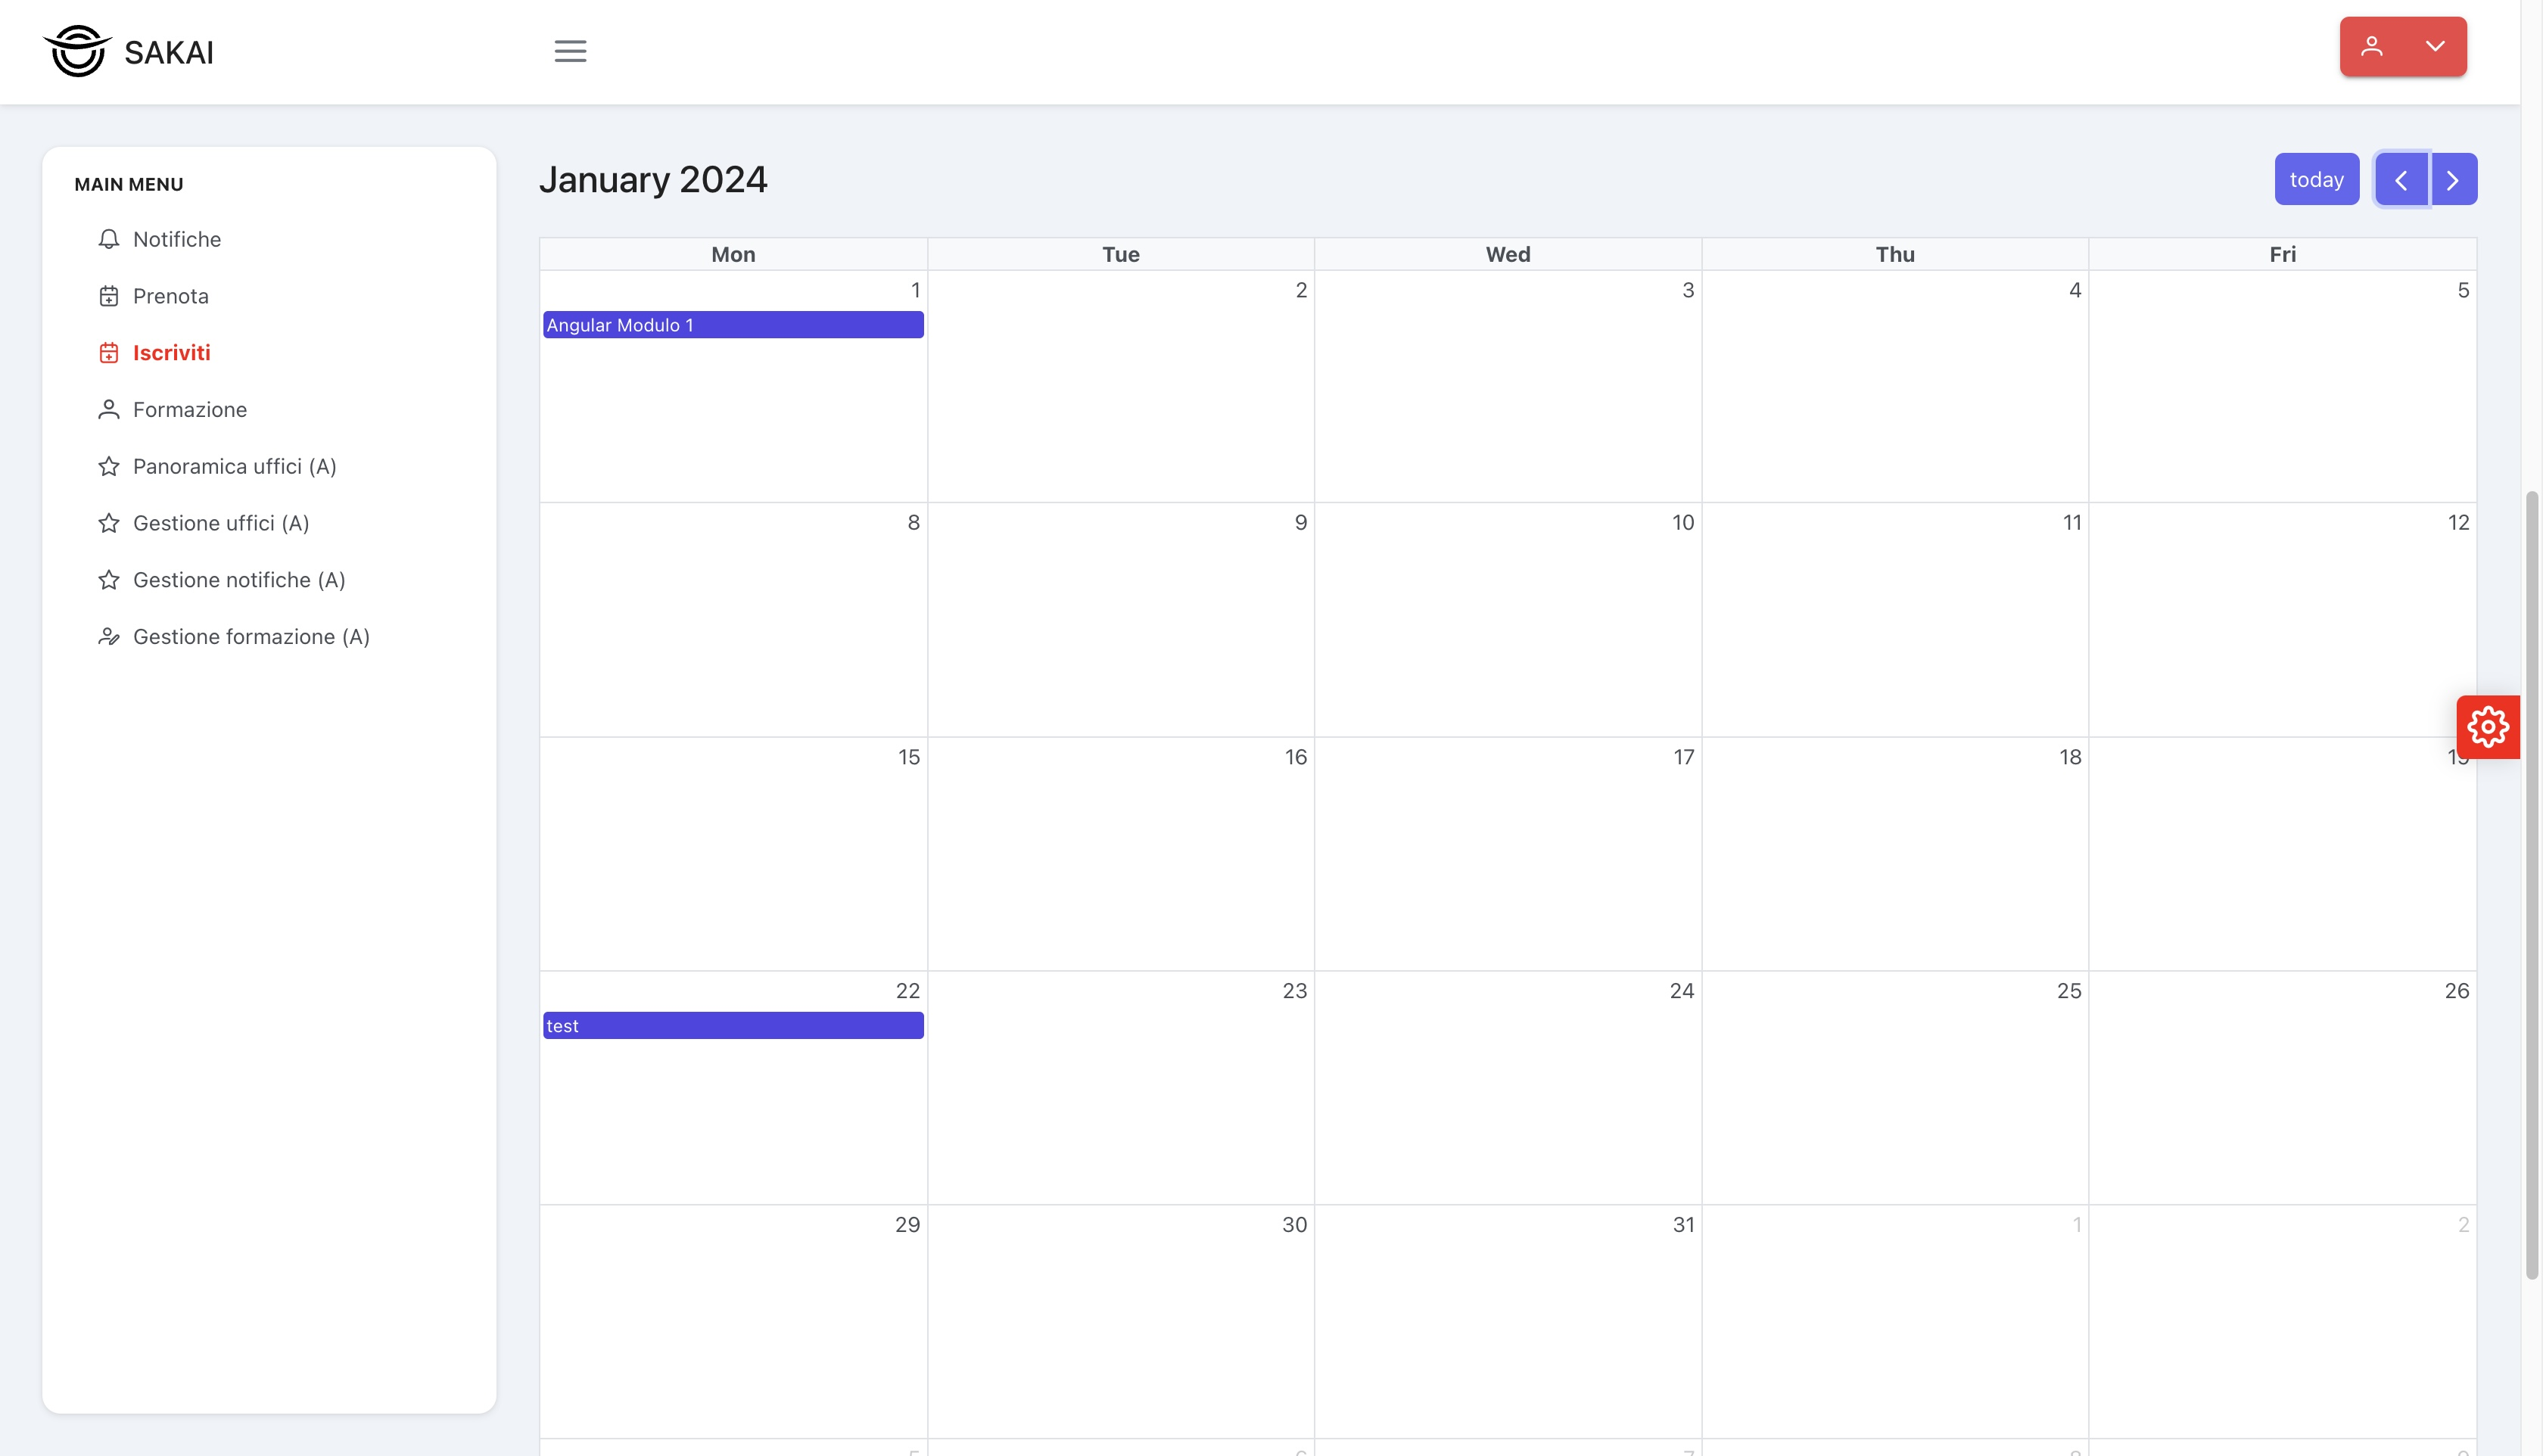
\includegraphics[width=1\textwidth]{fullcalendar.png}
TODO aggiungere screen fullcalendar
\caption{\label{fig:fullcalendar}Il calendario visibile a larghezza intera, il quale visualizza i corsi di formazione esistenti.}
\end{figure}

Dopo averlo installato tramite la \acrshort{cli} di \gls{angular}, ho dovuto configurare il file \texttt{app.component.ts} e \texttt{app.module.ts}, in modo da poterlo usare correttamente.
\begin{figure}[H]
\centering
\begin{lstlisting}[language=TYPESCRIPT, linewidth=20cm, basicstyle=\tiny]
export class AppComponent implements OnInit {
  calendarOptions: CalendarOptions = {
      initialView: 'dayGridMonth',
      plugins: [dayGridPlugin]
  };
...
}
\end{lstlisting}
\caption{\label{fig:fullcalendar module}Il codice \acrshort{ts} del file \texttt{app.module.ts}, necessario per il funzionamento del calendario.}
\end{figure}

Di seguito, il codice \acrshort{html} e \acrshort{ts} per gestire la logica di business del componente \texttt{fullcalendarComponent}:
\begin{figure}[H]
\centering
\begin{lstlisting}[language=HTML, linewidth=20cm, basicstyle=\tiny]
<full-calendar [options]="calendarOptions"></full-calendar>
\end{lstlisting}
\caption{\label{fig:fullcalendar.html}Il codice \acrshort{html} del file \texttt{fullcalendar.component.html}.}
\end{figure}

\begin{figure}[H]
\centering
\begin{lstlisting}[language=TypeScript, linewidth=20cm, basicstyle=\tiny]
ngOnInit(): void {
  this.coursesData$ = this.store.select(selectCoursesData).pipe(startWith(this.route.snapshot.data.CoursesData));
  this.coursesData$.pipe(
      filter(data => !!data)
  ).subscribe((data) => {
      this.totalRecords$ = this.coursesData$.pipe(map((x) => (x ? (x[0] ? x[0].count : 0) : 0)));

      let tmp = [];
      data.forEach((course) => {
          let day:string = course.coursesDate[0] + course.coursesDate[1];
          let month:string = course.coursesDate[3] + course.coursesDate[4];
          let year:string = course.coursesDate[6] + course.coursesDate[7] + course.coursesDate[8] + course.coursesDate[9];

          tmp.push({ title: course.coursesName, date: year + '-' + month + '-' + day }); // yyy-mm-dd
          console.log(tmp);
      });

      this.calendarOptions = {
          ...this.calendarOptions,
          events: tmp
      };
  })
}
\end{lstlisting}
\caption{\label{fig:fullcalendar.ts}Il codice TypeScript del file \texttt{education.component.ts}, necessario per il funzionamento della logica di business del calendario.}
\end{figure}



Infine, è stato necessario sviluppare i file mancanti per il completo funzionamento del progetto di prova finale, quindi i file per la gestione ti tutti i componenti restanti, in modo da l'applicazione web potesse gestire correttamente la visualizzazione, la modifica, la ricerca, l'aggiunta e la cancellazione dei corsi di formazione da parte dell'admin e la visualizzazione dei corsi di formazione da parte dell'utente base. 
Inoltre, in fase finale del tirocinio, ho aggiunto un componente per la gestione delle iscrizioni da parte degli utenti base. 
Le figure dei codici, dei file sopra citati, sono omesse, in quanto sono consone al codice già mostrato e descritto in precedenza.\newline


\subsection{PrimeNG}\label{subsec:primeng}
% Una veloce digressione su PrimeNG e su come l'ho usato e perchè \dots\newline
Grazie a \acrshort{primeng}, ho potuto implementare una \acrshort{gui} funzionale e minimalistica.
Innanzitutto, è stato necessario installare i giusti pacchetti e le giuste dipendenze, tramite \acrshort{cli}, successivamenteme, la scelta dei componenti utilizzati e descritti in precedenza, è stata fatta in base alle esigenze del progetto e alle funzionalità offerte da \acrshort{primeng}.
In particolare, i componenti usati sono:
\begin{itemize}
  \item \texttt{p-table}, per la visualizzazione dei corsi di formazione;
  \item \texttt{p-sortableColumn} e \texttt{p-sortIcon}, per l'ordinamento dei dati della tabella;
  \item \texttt{p-inputText}, \texttt{p-dropdown}, \texttt{p-calendar}, per la gestione dei campi di input e delle date;
  \item \texttt{p-button}, per la gestione dei pulsanti di modifica e cancellazione;
  \item \texttt{p-fullCalendar}, per la visualizzazione dei corsi di formazione esistenti in un calendario.
  \item \texttt{ngtemplate}, per la gestione dei template personalizzati.
\end{itemize}

Di seguito, un esempio di come è stato usato il componente \texttt{ng} per la visualizzazione dei corsi di formazione:
\begin{figure}[H]
\centering
\begin{lstlisting}[language=HTML, linewidth=20cm, basicstyle=\tiny]
  <ng-template pTemplate="body" let-coursesData>
        <tr class="p-selectable-row" [pRowToggler]="coursesData.coursesId">
            <td>
                <button type="button" pButton pRipple
                    class="p-button-text p-button-rounded p-button-plain"
                    [icon]="isRowExpanded(coursesData.coursesId) ? 'pi pi-chevron-down' : 'pi pi-chevron-right'"
                    (click)="toggleRow(coursesData.coursesId)">
                </button>
            </td>
            <td>
                <span class="p-column-title">Nome corso</span>
                {{coursesData.coursesName}}
            </td>
            <td>
                <span class="p-column-title">Tipologia</span>
                {{coursesData.coursesType}}
            </td>
            <td>
                <span class="p-column-title">Data inizio</span>
                {{coursesData.coursesDate}}
            </td>
            <td>
                <span class="p-column-title">Prenota</span>
                <p-button icon="pi pi-check" (click)="addEnrollment(coursesData);"></p-button>
            </td>

        </tr>

        <tr>
        </tr>

        <tr *ngIf="isRowExpanded(coursesData.coursesId)">
            <td [attr.colspan]="globalFiltersFields.length + 1">
                <div class="expanded-content">
                    <p>immagine corso scelta con switch</p>
                </div>
            </td>
        </tr>
    </ng-template>
\end{lstlisting}
\caption{\label{fig:primeng ng}Il codice \acrshort{html} del file \texttt{education.component.html}, in particolare la tabella di \acrshort{primeng}.}
\end{figure}


\subsection{Servizi Angular}\label{subsec:servizi-angular}
% Una veloce digressione sui servizi Angular e come sono stati usati \dots\newline
I servizi \gls{angular} sono tra le funzionalità più potenti e flessibili del medesimo \gls{framework}, in quanto permettono di creare e gestire la logica di business in modo efficiente e modulare. Durante questo tirocinio di prova finale, sono stati usati al fine di gestire la comunicazione tra il livello di presentazione e il livello della logica di business. Inoltre, sono stati scelti per la loro capacità di essere iniettati in qualsiasi componente.
Di seguito, un esempio di come è stato usato un servizio \gls{angular} per la gestione dei corsi di formazione:
\begin{figure}[H]
\centering
\begin{lstlisting}[language=TypeScript, linewidth=20cm, basicstyle=\tiny]
  @Injectable({ providedIn: "root" })
\end{lstlisting}
\caption{\label{fig:angular service}Il codice \acrshort{ts} del file \texttt{course.resolver.ts}, contenente l'implementazione di un servizio \gls{angular}.}
\end{figure}

\begin{figure}[H]
\centering
\begin{lstlisting}[language=TypeScript, linewidth=20cm, basicstyle=\tiny]
  @Injectable({ providedIn: "any" })
\end{lstlisting}
\caption{\label{fig:angular service 2}Il codice \acrshort{ts} del file \texttt{admin-user-guard.ts}, contenente l'implementazione di un servizio \gls{angular}.}
\end{figure}

% `